%%%%%%%%%%%%%%%%%%%%%%%%%%%%%%%%%%%%%%%%%
% Masters/Doctoral Thesis 
% LaTeX Template
% Version 1.43 (17/5/14)
%
% This template has been downloaded from:
% http://www.LaTeXTemplates.com
%
% Original authors:
% Steven Gunn 
% http://users.ecs.soton.ac.uk/srg/softwaretools/document/templates/
% and
% Sunil Patel
% http://www.sunilpatel.co.uk/thesis-template/
%
% License:
% CC BY-NC-SA 3.0 (http://creativecommons.org/licenses/by-nc-sa/3.0/)
%
% Note:
% Make sure to edit document variables in the Thesis.cls file
%
%%%%%%%%%%%%%%%%%%%%%%%%%%%%%%%%%%%%%%%%%

%----------------------------------------------------------------------------------------
%	PACKAGES AND OTHER DOCUMENT CONFIGURATIONS
%----------------------------------------------------------------------------------------

\documentclass[11pt, oneside]{Thesis} % The default font size and one-sided printing (no margin offsets)

\graphicspath{{Pictures/}} % Specifies the directory where pictures are stored
\usepackage{times}
\usepackage{pdfpages}
\usepackage{subfigure}
\usepackage[square, numbers, comma, sort&compress]{natbib} % Use the natbib reference package - read up on this to edit the reference style; if you want text (e.g. Smith et al., 2012) for the in-text references (instead of numbers), remove 'numbers' 
\usepackage{amsmath}
\usepackage{amssymb}
\usepackage{graphicx}
\usepackage{listings}

\hypersetup{urlcolor=blue, colorlinks=true} % Colors hyperlinks in blue - change to black if annoying
\title{\ttitle} % Defines the thesis title - don't touch this

\begin{document}
\frontmatter % Use roman page numbering style (i, ii, iii, iv...) for the pre-content pages

\setstretch{1.3} % Line spacing of 1.3

% Define the page headers using the FancyHdr package and set up for one-sided printing
\fancyhead{} % Clears all page headers and footers
\rhead{\thepage} % Sets the right side header to show the page number
\lhead{} % Clears the left side page header

\pagestyle{fancy} % Finally, use the "fancy" page style to implement the FancyHdr headers

\newcommand{\HRule}{\rule{\linewidth}{0.5mm}} % New command to make the lines in the title page
\newcommand{\datasetunimore} {Interactive Museum}
\newcommand{\argmax}{\arg\!\max}
% PDF meta-data
\hypersetup{pdftitle={\ttitle}}
\hypersetup{pdfsubject=\subjectname}
\hypersetup{pdfauthor=\authornames}
\hypersetup{pdfkeywords=\keywordnames}

%----------------------------------------------------------------------------------------
%	TITLE PAGE
%----------------------------------------------------------------------------------------

\begin{titlepage}

\begin{center}
\textsc{\Large \bf \univname}\\[0.5cm] % University name
\textsc{\large Dipartimento di Ingegneria ``Enzo Ferrari"}\\[0.2cm] % Thesis type
%\HRule \\ % Horizontal line
\textsc{\large Corso di Laurea Magistrale in Ingegneria Informatica}\\[5.5cm] % Thesis type

\HRule \\[0.4cm] % Horizontal line
{\huge \bfseries \ttitle}\\[0.4cm] % Thesis title
\HRule \\[1.5cm] % Horizontal line
 
\begin{minipage}{0.4\textwidth}
\begin{flushleft} \large
\emph{Candidato:}\\
\authornames % Author name - remove the \href bracket to remove the link
\end{flushleft}
\end{minipage}
\begin{minipage}{0.4\textwidth}
\begin{flushright} \large
\emph{Relatore:} \\
\supname \\ % Supervisor name - remove the \href bracket to remove the link  
\emph{Correlatore:} \\
\cosupname \\ % Supervisor name - remove the \href bracket to remove the link  
\end{flushright}
\end{minipage}\\[5.5cm]
 
%\large \textit{A thesis submitted in fulfilment of the requirements\\ for the degree of \degreename}\\[0.3cm] % University requirement text
%\textit{in the}\\[0.4cm]
%\groupname\\\deptname\\[2cm] % Research group name and department name
 
\textsc{\large Anno Accademico 2013-2014}\\[4cm] % Date
%\includegraphics{Logo} % University/department logo - uncomment to place it
 
\vfill
\end{center}

\end{titlepage}

%----------------------------------------------------------------------------------------
%	DECLARATION PAGE
%	Your institution may give you a different text to place here
%----------------------------------------------------------------------------------------

%\Declaration{
%
%\addtocontents{toc}{\vspace{1em}} % Add a gap in the Contents, for aesthetics
%
%I, \authornames, declare that this thesis titled, '\ttitle' and the work presented in it are my own. I confirm that:
%
%\begin{itemize} 
%\item[\tiny{$\blacksquare$}] This work was done wholly or mainly while in candidature for a research degree at this University.
%\item[\tiny{$\blacksquare$}] Where any part of this thesis has previously been submitted for a degree or any other qualification at this University or any other institution, this has been clearly stated.
%\item[\tiny{$\blacksquare$}] Where I have consulted the published work of others, this is always clearly attributed.
%\item[\tiny{$\blacksquare$}] Where I have quoted from the work of others, the source is always given. With the exception of such quotations, this thesis is entirely my own work.
%\item[\tiny{$\blacksquare$}] I have acknowledged all main sources of help.
%\item[\tiny{$\blacksquare$}] Where the thesis is based on work done by myself jointly with others, I have made clear exactly what was done by others and what I have contributed myself.\\
%\end{itemize}
% 
%Signed:\\
%\rule[1em]{25em}{0.5pt} % This prints a line for the signature
% 
%Date:\\
%\rule[1em]{25em}{0.5pt} % This prints a line to write the date
%}

\clearpage % Start a new page

%----------------------------------------------------------------------------------------
%	QUOTATION PAGE
%----------------------------------------------------------------------------------------

%\pagestyle{empty} % No headers or footers for the following pages
%
%\null\vfill % Add some space to move the quote down the page a bit
%
%\textit{``Thanks to my solid academic training, today I can write hundreds of words on virtually any topic without possessing a shred of information, which is how I got a good job in journalism."}
%
%\begin{flushright}
%Dave Barry
%\end{flushright}
%
%\vfill\vfill\vfill\vfill\vfill\vfill\null % Add some space at the bottom to position the quote just right
%
%\clearpage % Start a new page

%----------------------------------------------------------------------------------------
%	ABSTRACT PAGE
%----------------------------------------------------------------------------------------

%\addtotoc{Abstract} % Add the "Abstract" page entry to the Contents
%
%\abstract{\addtocontents{toc}{\vspace{1em}} % Add a gap in the Contents, for aesthetics
%
%The Thesis Abstract is written here (and usually kept to just this page). The page is kept centered vertically so can expand into the blank space above the title too\ldots
%}
%
\clearpage % Start a new page

%----------------------------------------------------------------------------------------
%	DEDICATION
%----------------------------------------------------------------------------------------
\mainmatter
\setstretch{1.3} % Return the line spacing back to 1.3

\pagestyle{empty} % Page style needs to be empty for this page

\dedicatory{To Emanuela} % Dedication text

\addtocontents{toc}{\vspace{2em}} % Add a gap in the Contents, for aesthetics

%----------------------------------------------------------------------------------------
%	ACKNOWLEDGEMENTS
%----------------------------------------------------------------------------------------

\setstretch{1.3} % Reset the line-spacing to 1.3 for body text (if it has changed)

\acknowledgements{\addtocontents{toc}{\vspace{1em}} % Add a gap in the Contents, for aesthetics

Foremost, I would like to express my sincere gratitude to my advisors Prof. Rita Cucchiara and Dr. Giuseppe Serra for the continuous support of my study, for their patience, motivation, enthusiasm, and knowledge. Their guidance helped me in all the time of research and writing of this thesis. I could not have imagined having better advisors for my study.

Besides my advisors, I would like to thank the rest of the Imagelab research group: Costantino Grana, Simone Calderara, Michele Fornaciari, Marco Manfredi, Paolo Santinelli, Augusto Pieracci, Roberto Vezzani, Franesco Solera, Martino Lombardi and Patrizia Varini, for their encouragement, insightful comments, and hard questions. I am also grateful to Prof. Greg Mori, for enlightening me the first glance of research during a visit in Modena.

Special thanks go to my labmates Stefano Alletto and  Francesco Paci, for the stimulating discussions, for the days we were working together before deadlines, and for all the fun we have had in the last months. Also I thank my friends Chiara Ferrari, Emanuele Benatti, Xhensila Doda, Davide Setti, and in particular Michela Benedetti, who encouraged me to study computer vision.

Last but not the least, I would like to thank my parents Franco and Elisabetta, for giving birth to me at the first place and supporting me throughout my life, and my sister Alessia.
}
\clearpage % Start a new page

%----------------------------------------------------------------------------------------
%	LIST OF CONTENTS/FIGURES/TABLES PAGES
%----------------------------------------------------------------------------------------

\pagestyle{fancy} % The page style headers have been "empty" all this time, now use the "fancy" headers as defined before to bring them back

\lhead{\emph{Contents}} % Set the left side page header to "Contents"
\tableofcontents % Write out the Table of Contents

\lhead{\emph{List of Figures}} % Set the left side page header to "List of Figures"
\listoffigures % Write out the List of Figures

\lhead{\emph{List of Tables}} % Set the left side page header to "List of Tables"
\listoftables % Write out the List of Tables

%----------------------------------------------------------------------------------------
%	ABBREVIATIONS
%----------------------------------------------------------------------------------------

%\clearpage % Start a new page
%
%\setstretch{1.5} % Set the line spacing to 1.5, this makes the following tables easier to read
%
%\lhead{\emph{Abbreviations}} % Set the left side page header to "Abbreviations"
%\listofsymbols{ll} % Include a list of Abbreviations (a table of two columns)
%{
%\textbf{LAH} & \textbf{L}ist \textbf{A}bbreviations \textbf{H}ere \\
%%\textbf{Acronym} & \textbf{W}hat (it) \textbf{S}tands \textbf{F}or \\
%}

%----------------------------------------------------------------------------------------
%	PHYSICAL CONSTANTS/OTHER DEFINITIONS
%----------------------------------------------------------------------------------------

%\clearpage % Start a new page
%
%\lhead{\emph{Physical Constants}} % Set the left side page header to "Physical Constants"
%
%\listofconstants{lrcl} % Include a list of Physical Constants (a four column table)
%{
%Speed of Light & $c$ & $=$ & $2.997\ 924\ 58\times10^{8}\ \mbox{ms}^{-\mbox{s}}$ (exact)\\
%% Constant Name & Symbol & = & Constant Value (with units) \\
%}

%----------------------------------------------------------------------------------------
%	SYMBOLS
%----------------------------------------------------------------------------------------

%\clearpage % Start a new page
%
%\lhead{\emph{Symbols}} % Set the left side page header to "Symbols"
%
%\listofnomenclature{lll} % Include a list of Symbols (a three column table)
%{
%$a$ & distance & m \\
%$P$ & power & W (Js$^{-1}$) \\
%% Symbol & Name & Unit \\
%
%& & \\ % Gap to separate the Roman symbols from the Greek
%
%$\omega$ & angular frequency & rads$^{-1}$ \\
%% Symbol & Name & Unit \\
%}
\newcommand{\etal}{\textit{et al.~}}
%----------------------------------------------------------------------------------------
%	THESIS CONTENT - CHAPTERS
%----------------------------------------------------------------------------------------

 % Begin numeric (1,2,3...) page numbering

\pagestyle{fancy} % Return the page headers back to the "fancy" style

% Include the chapters of the thesis as separate files from the Chapters folder
% Uncomment the lines as you write the chapters

% Chapter 1

\chapter{Wearable devices and new human-machine interfaces: an overview}

\lhead{Chapter 1. \emph{Wearable devices and new human-machine interfaces}} % This is for the header on each page - perhaps a shortened title

%----------------------------------------------------------------------------------------

\section{Where to wear an extra eye?}
Positioning an optical device on the human body is quite a problematic task, as occlusion, motion, social issues as well as criteria related to the purpose of the device must be taken into account.\footnote{\url{http://www.robots.ox.ac.uk/~wmayol/3D/nancy_matlab.html}}. Following the work of Mayol \etal \cite{mayol2001positioning}, in this section we give a detailed overview on the best places where to put a wearable camera.

Cameras used for wearable applications fall into two categories for this discussion; static narrow-view devices and omnidirectional devices. Omnidirectional devices include catadioptric, fish-eye and active systems where either the entire field-of-viewis imaged at low resolution, or in the active case the high-resolution narrow-view sensor moved to any orientation. Narrow-view static cameras can only ever see a small part of the user or their environment, and placement is therefore entirely driven by the task. For wide-angle or omnidirectional sensors placement is less constrained and a range of positions are possible. 

A variety of solutions appear in the literature. In \cite{starner1998real, schiele1999attentional}, hat-mounted cameras have been used to look down at the user’s hands and reaching space, whereas in [9, 13] cameras are strapped to the wearer’s hands themselves. In [10], a hat-mounted camera looks forward, an orientation also used when the camera is attached to a head mounted display [2]. In contrast, [11, 6] uses a camera worn on the chest, in [5] an omnidirectional camera is used above the head, and a wide-angle lens camera mounted at the back in [12] and in previous work [4] we placed a miniature active vision system on the shoulder.
In a previous paper [4], we identified three frames of reference for measurements that a wearable sensor makes: I relative to the user body (e.g. sensing the manipulative space in front of the user’s chest) II relative to the static world (e.g. sensing the ceiling/
floor texture to infer user’s location)
III relative to an independent object (e.g. tracking an interesting
object)
This task-oriented classification can help us to understand
the criteria that should be considered. For working
in the user frame alone all that is required is a stable view
of the chosen area — often the handling space, and absolute
field-of-view may be less important. For sensing the
outside environment user occlusion is problematic and absolute
field-of-view is more important. Both occlusion and
user motion are problems when fixating resolution or processing
on a particular part of the environment or independently
moving object.


\begin{figure}[htbp]
	\centering
		\includegraphics[page=3]{Figures/mayol_etal_ouel224101_cropped.pdf}
	\caption[An Electron]{An electron (artist's impression).}
	\label{fig:Electron}
\end{figure}

\begin{figure}[htbp]
	\centering
		\includegraphics[page=4]{Figures/mayol_etal_ouel224101_cropped.pdf}
	\caption[An Electron]{An electron (artist's impression).}
	\label{fig:Electron}
\end{figure}

\begin{figure}[htbp]
	\centering
		\includegraphics[page=5]{Figures/mayol_etal_ouel224101_cropped.pdf}
	\caption[An Electron]{An electron (artist's impression).}
	\label{fig:Electron}
\end{figure}

%----------------------------------------------------------------------------------------

\section{Gestures}
Gestures are expressive, meaningful body motions involving
physical movements of the fingers, hands, arms, head, face, or
body with the intent of conveying meaningful information
or interacting with the environment. They constitute one interesting
small subspace of possible human motion. A gesture
may also be perceived by the environment as a compression
technique for the information to be transmitted elsewhere and
subsequently reconstructed by the receiver. Gesture recognition
has wide-ranging applications such as the following:
\begin{itemize}
\item developing aids for the hearing impaired;
\item  enabling very young children to interact with computers;
\item  designing techniques for forensic identification;
\item recognizing sign language;
\item medically monitoring patients’ emotional states or stress
levels;
\item lie detection;
\item navigating and/or manipulating in virtual environments;
\item communicating in video conferencing;
\item distance learning/tele-teaching assistance;
\item monitoring automobile drivers' alertness/drowsiness
levels, etc.
\end{itemize}

Generally, there exist many-to-one mappings from concepts
to gestures and vice versa. Hence, gestures are ambiguous and
incompletely specified. For example, to indicate the concept
\textit{stop}, one can use gestures such as a raised hand with palm
facing forward, or, an exaggerated waving of both hands over the
head. Similar to speech and handwriting, gestures vary between
individuals, and even for the same individual between different
instances.

Gestures can be static (the user assumes a certain pose or configuration)
or dynamic (with prestroke, stroke, and poststroke
phases). Some gestures also have both static and dynamic elements,
as in sign languages. Again, the automatic recognition
of natural continuous gestures requires their temporal segmentation.
Often one needs to specify the start and end points of a
gesture in terms of the frames of movement, both in time and
in space. Sometimes a gesture is also affected by the context of
preceding as well as following gestures. Moreover, gestures are
often language- and culture-specific. They can broadly be of the
following types:

%----------------------------------------------------------------------------------------

\section{In Closing}


% Chapter 1

\chapter{Computer Vision and Machine Learning techniques used in this thesis}

\lhead{Chapter 2. \emph{Computer Vision and Machine Learning techniques}} % This is for the header on each page - perhaps a shortened title

\section{Color spaces}
\section{Descriptors}
\subsection{Histograms of Oriented Gradient}
\subsection{Histograms of Optical Flow}
\subsection{MBH}
\subsection{Bag of Words}
The bag-of-words (BoW) methodology was first proposed in the text retrieval domain problem for text document analysis, and it was further adapted for computer vision applications \cite{bosch2007best}. For image analysis, a visual analogue of a word is used in the BoWmodel, which is based on the vector quantization process by clustering low-level visual features of local regions. 

To extract the BoW feature from images involves the following steps: 
\begin{enumerate}
\item automatically detect regions/points of interest,
\item compute local descriptors over those regions/points,
\item quantize the descriptors into words to form the visual vocabulary
\item find the occurrences in the image of each specific word in the vocabulary for constructing the BoW feature (or a histogram of word frequencies).
\end{enumerate}

\begin{figure}[htbp]
	\centering
		\includegraphics[page=3]{Figures/376804_cropped.pdf}
	\caption{The Bag of Words approach.}
	\label{fig:BoW}
\end{figure}

Figure \ref{fig:BoW} describes these four steps to extract the BoW feature from images. The BoW model can be defined as follows. Given a training dataset $D$ containing $n$ images represented by $D = d_1, d_2, \text{...}, d_n$, where $d$ is the extracted visual features, a specific unsupervised learning algorithm, such as k-means, is used to group $D$ based on a fixed number of visual words $W$ (or categories) represented by $W = w_1,w_2, \text{...}, w_K$, where $K$ is the number of clusters. Then, we can summarize the data in a $K\times N$ cooccurrence table of counts $N_{i j} = n(w_i, d_j )$, where $n(w_i, d_j)$ denotes how often the word $w_i$ occurred in an image $d_i$. The $i$-th column of this table can be used as a global descriptor for the $i$-th image: thanks to the clustering phase a fixed-size descriptor has been obtained from a variable number of points of interests and thus from a variable number of local descriptors.

As stated before, the traditional application of the Bag of Words approach is image classification. Usually SIFT keypoints and descriptors are extracted, and BoW histograms are then passed to a SVM classifier. However, the same principle can be used to classify videos or frame sequences, if we employ spatio-temporal points of interest and descriptors: in the following of this thesis, the BoW technique will be used in combination with spatio-temporal trajectories extracted from frame sequences, each described in its shape and appearance. We will then be able to classify frame sequences instead of images, and to have a descriptor with fixed length even in presence of a variabile number of trajectories per frame. Other techinques will be then proposed to deal with actions with variable length (and thus described by a variable number of frames).


\section{Support Vector Machines classifiers}
The last step in the traditional computer vision pipeline is classification: in this thesis, we will employ the Support Vector Machine classifier, both in its linear version and in its structured version. Support Vector Machines (SVM) have been one of the most popular classifiers in recent years for solving problems in classification, regression, and novelty detection. An important property of support vector machines is that the determination of the model parameters corresponds to a convex optimization problem, and so any local solution is also a global optimum.

\subsection{Linear SVMs}
Let's start with the simplest case: linear support vector machines trained on separable data. Label the training data $\{ \mathbf{x}_i, y_i\}$ $i=1, ..., l$, $y_i \in \{-1,1\}$, $\mathbf{x}_i \in \mathbb{R}^d$. Suppose we have some hyperplane which separates the positive from the negative samples. The points $\mathbf{x}$ which lie on the hyperplane satisfy $\mathbf{w} \cdot \mathbf{x} + b = 0$, where $\mathbf{w}$ is normal to the hyperplane, $|b|/\|\mathbf{w}\|$ is the perpendicular distance from the hyperplane to the origin and $\|\mathbf{w}\|$ is the Euclidean norm of $\mathbf{w}$. Let $\mathbf{w} \cdot \mathbf{x} +b = a$ ($\mathbf{w} \cdot \mathbf{x} +b = -a$) be the hyperplane that touches the closest positive (negative) example. Define the \textit{margin} of a separable hyperplane to be $2a / \| \mathbf{w} \|$. For the linearly separable case, the support vector algorithm simply looks for the separating hyperplane with the largest margin. This can be formulated as follows: suppose that all the training data satisfy the following constraints:

\begin{equation}
\mathbf{w} \cdot \mathbf{x}_i + b \ge +1 \quad \text{if } y_i = +1
\label{const1}
\end{equation}
\begin{equation}
\mathbf{w} \cdot \mathbf{x}_i + b \le -1 \quad \text{if } y_i = -1
\label{constr2}
\end{equation}

We will now switch to a Lagrangian formulation of the problem. There are two reasons
for doing this. The first is that the constraints will be replaced by constraints on the
Lagrange multipliers themselves, which will be much easier to handle. The second is that
in this reformulation of the problem, the training data will only appear (in the actual training
and test algorithms) in the form of dot products between vectors. This is a crucial property
which will allow us to generalize the procedure to the nonlinear case.

Thus, we introduce positive Lagrange multipliers $\alpha_i$, $i = 1, ... , l$, one for each of the
inequality constraints (\ref{ineq-constr}). For constraints of the form $c_i \ge 0$, as in our case, the
constraint equations are multiplied by positive Lagrange multipliers and subtracted from the objective function, to form the Lagrangian. For equality constraints, the Lagrange multipliers are unconstrained. This gives Lagrangian:
\begin{equation}
L_p = \frac{1}{2} \| \mathbf{w} \|^2 - \sum_{i=1}^l \alpha_i y_i (\mathbf{x}_i \cdot \mathbf{w} + b) + \sum_{i=1}^l \alpha_i
\label{Lp}
\end{equation}

We must now minimize $L_p$ with respect to $\mathbf{w}$, $b$, and simultaneously require that the
derivatives of $L_p$ with respect to all the $\alpha_i$ vanish, all subject to the constraints $\alpha_i \ge 0$. Now this is a convex quadratic programming
problem, and those points which satisfy the
constraints also form a convex set. Requiring that the gradient of $L_p$ with respect to $\mathbf{w}$ and $b$ vanish give the conditions:
\begin{equation}
\frac{\partial L_p}{\partial \mathbf{w}} = 0 \Longleftrightarrow \mathbf{w} = \sum_{i=1}^l \alpha_i y_i \mathbf{x}_i
\label{14}
\end{equation}

\begin{equation}
\frac{\partial L_p}{\partial b} = 0 \Longleftrightarrow \sum_{i=1}^l \alpha_i y_i =0
\label{15}
\end{equation}

We can substitute these equalities into (\ref{Lp}) to give:
\begin{equation}
L_d=  \sum_{i} \alpha_i - \frac{1}{2} \sum_{i,j} \alpha_i\alpha_j y_iy_j \mathbf{x}_i \cdot \mathbf{x}_j
\end{equation}
Support vector training (for the separable, linear case) therefore amounts to maximizing
$L_d$ with respect to the $\alpha_i$, subject to constraints (\ref{15}) and positivity of the $\alpha_i$, with solution
given by (\ref{14}). Notice that there is a Lagrange multiplier $\alpha_i$ for every training point. In
the solution, those points for which $\alpha_i > 0$ are called \textit{support vectors}.

Since not always the training data is linearly separable, we would like to relax the constraints (\ref{const1}) and (\ref{constr2}), but only when necessary, that is, we would like to introduce a further cost for
doing so. This can be done by introducing positive slack variables $\epsilon_i$, $i = 1, ... , l$ in the
constraints \cite{cortes1995support}, which then become:

\begin{equation}
\mathbf{w} \cdot \mathbf{x}_i + b \ge +1 \quad \text{if } y_i = +1 - \epsilon_i
\label{const1b}
\end{equation}
\begin{equation}
\mathbf{w} \cdot \mathbf{x}_i + b \le -1 \quad \text{if } y_i = -1 + \epsilon_i
\label{constr2b}
\end{equation}

Thus, for an error to occur, the corresponding $\epsilon_i$ must exceed unity. Combining the two inequalities, and adding an extra cost for errors to the objective function, we can formulate the problem of margin maximization as:
\begin{equation}
\min_{\mathbf{w},b} \mathbf{w}\cdot\mathbf{w} + C \sum_{i=1}^l \epsilon_i \quad \text{s.t.  }
y_i(\mathbf{w} \cdot \mathbf{x}_i + b)-1 + \epsilon_i \ge 0
\label{ineq-constr}
\end{equation}
where $C$ is a parameter to be chosen by the user, a larger $C$ corresponding to assigning
a higher penalty to error.

\subsection{Structured Learning and Structured SVM}
Structured learning deals with the general problem of learning a mapping
from input vectors or patterns $\mathbf{x}\in\mathcal{X}$ to discrete
response variables $\mathbf{y}\in\mathcal{Y}$, based on a training
sample of input-output pairs $(\mathbf{x}_{1},\mathbf{y}_{1}),\ldots,(\mathbf{x}_{n},\mathbf{y}_{n})\in\mathcal{X}\times\mathcal{Y}$
drawn from some fixed but unknown probability distribution. Unlike
multiclass classification, where the output space consists of an arbitrary
finite set of labels or class identifiers, structured classification
considers the case where the elements of $\mathcal{Y}$ are structured
objects such as sequences, strings, trees, images or graphs. 

The objective of a structured classifier is thus to learn functions $f:\mathcal{X}\rightarrow\mathit{\mathcal{Y}}$
between the input space and arbitrary discrete output spaces, based
on a training sample of input-output pairs, and the approach we pursue
is to learn a discriminant function $F:\mathcal{X}\times\mathit{\mathcal{Y}\rightarrow\mathbb{R}}$
over input-output pairs from which we can derive a prediction by maximizing
$F$ over the response variable for a specific given input $\mathbf{x}$. Hence, the general form of our hypotheses $f$ is

\begin{equation}
f(\mathbf{x},\mathbf{y}) =\argmax_{\mathbf{y} \in \mathcal{Y}} F(\mathbf{x},\mathbf{y};\mathbf{w})
\end{equation}

where $\mathbf{w}$ denotes a parameter vector. $F$ can be thought as a compatibility function that measures how compatible pairs $(\mathbf{x},\mathbf{y})$ are. We can assume $F$ to be linear in some combined feature representation of input and outputs $\Phi(\mathbf{x},\mathbf{y})$:

\begin{equation}
F(\mathbf{x},\mathbf{y};\mathbf{w}) = \langle \mathbf{w}, \Phi(\mathbf{x},\mathbf{y}) \rangle
\end{equation}

where the specific form of $\Phi(\mathbf{x},\mathbf{y})$ depends on the nature of the problem.

We then define a loss function $\Delta : \mathcal{Y} \times \mathcal{Y} \rightarrow \mathbb{R}$, where $\Delta(\mathbf{y},\mathbf{y'})$ quantifies the loss associated with a prediction $\mathbf{y'}$ if the true output value is $\mathbf{y}$. If we assume that input-output pairs $(\mathbf{x},\mathbf{y})$ are generated according to some fixed distribution $P(\mathbf{x},\mathbf{y})$, we could describe the goal of supervised learning as to find a function $f$ that minimizes the following risk

\begin{equation}
\mathcal{R}^\Delta_P(f) = \int_{\mathcal{X} \times \mathcal{Y}} \Delta(\mathbf{y},f(\mathbf{x})) dP(\mathbf{x},\mathbf{y})
\end{equation}

but since $P$ is unknown, and we only have a finite training set of pairs $S = \{ (\mathbf{x}_i,\mathbf{y}_i) \in \mathcal{X}\times\mathcal{Y} : i=1,...,n\}$, we can describe the performance of a function $f$ on the training set $S$ by the empirical risk,

\begin{equation}
\mathcal{R}^\Delta_S(f) = \frac{1}{n} \sum_{i=1}^n \Delta(\mathbf{y}_i,f(\mathbf{x_i}))
\end{equation}

First, we consider the separable case in which there exists a function $f$ parameterized by $\mathbf{w}$ such that the empirical risk is zero. If we assume that $\Delta(\mathbf{y}, \mathbf{y'}) > 0$ for $\mathbf{y} \neq \mathbf{y'}$ and $\Delta(\mathbf{y}, \mathbf{y}) = 0$, then the condition of zero training error can then be compactly written as a set of non-linear constraints

\begin{equation}
\forall i: \max_{\mathbf{y} \in \mathcal{Y}-{\mathbf{y}_i}} \{ \langle \mathbf{w}, \mathbf{\Psi}(\mathbf{x}_i, \mathbf{y}) \rangle\} < \langle \mathbf{w}, \mathbf{\Psi}(\mathbf{x}_i,\mathbf{y}_i\rangle
\label{eq:for}
\end{equation}

Each nonlinear inequalities in \ref{eq:for} can be equivalently replaced by $|\mathcal{Y}|-1$ linear inequalities, resulting in a total of $n|\mathcal{Y}| -n$ linear constraints, 

\begin{equation}
\forall i, \forall \mathbf{y} \in \mathcal{Y}-\mathbf{y}_i: \langle \mathbf{w}, \delta\mathbf{\Psi}_i(\mathbf{y}) \rangle > 0
\label{eq:five}
\end{equation}

where we have defined the shorthand $\delta\mathbf{\Psi}_i(\mathbf{y}) =  \mathbf{\Psi}(\mathbf{x}_i, \mathbf{y}_i) -  \mathbf{\Psi}(\mathbf{x}_i, \mathbf{y})$.

If the set of inequalities in \ref{eq:five} is feasible, there will typically be more than one solution $\mathbf{w}^*$. To specify a unique solution, we propose to select $\mathbf{w}$ with $||\mathbf{w}||\leq 1$ for which the score of the correct label $\mathbf{y}_i$ is uniformly most different from the closest runnerup $\hat{\mathbf{y}_i}(\mathbf{w}) = \argmax_{\mathbf{y} \neq \mathbf{y}_i} \langle \mathbf{w}, \mathbf{\Psi}(\mathbf{x}_i, \mathbf{y})\rangle$. This generalizes the maximum-margin principle employed in SVMs to the more general case of structured learning. The resulting hard-margin optimization problem is:

\begin{equation} 
\min_{\mathbf{w}} \frac{1}{2} \lVert \mathbf{w} \rVert^2 \quad \text{s.t.} \forall i, \forall \mathbf{y} \in \mathcal{Y}-\{\mathbf{y}_i\}: \langle \mathbf{w},\delta\Psi_i(\mathbf{y}) \geq 1
\end{equation}

To allow errors in the training set slack variable are introduced and a soft-margin criterion is used. We introduce one slack variable for every non-linear constraint, which will result in an upper bound on the empirical risk and offers some additional algorithmic advantages. Adding a penalty term that is linear in the slack variables to the objective results in the quadratic program
\begin{eqnarray} \label{eq:svm}
\min_{\mathbf{w},\mathbf{\xi}} \frac{1}{2} \lVert \mathbf{w} \rVert^2 + \frac{C}{n} \sum_{i=1}^n \xi_i \nonumber \\
\text{s.t.} \forall i, \forall\xi_i \geq 0, \forall \mathbf{y} \in \mathcal{Y}-\{\mathbf{y}_i\}: 
\langle \mathbf{w},\delta\Psi_i(\mathbf{y})\rangle \geq 1 - \xi_i
\end{eqnarray}

However, also slack re-scaling can be used. Furthermore mn-slack and 1-slack versions have been proposed.

\subsection{Label Sequence Learning}
\label{svmhmm}
A special case of the general scenario of Structured learning is the problem of label sequence learning, or sequence annotation. Here the goal is to predict a label sequence $\mathbf{y} = (y^1,...,y^T)$ for a given observation sequence $\mathbf{x} = (\mathbf{x}^1,...,\mathbf{x}^T)$. If we assume that all sequences are of the same length $T$ and that $\mathbf{\Sigma}$ is the set of possible labels for each individual variable $y^t$, hence each sequence of labels is considered to a class of its own, resulting in a multiclass classification problem with $|\mathbf{\Sigma}|^T$ different classes. To model label sequence learning in this manner would of course not be very useful, if one were to apply standard multiclass classification methods.

Inspired by hidden Markov models (HMM) interactions, Altun \etal \cite{altun2003hidden} propose to define $\Psi$ to include interactions between input features and labels via multiple copies of the input features as well as features that model interactions between nearby label variables. Before modeling the discriminant function $F$, we need to define the canonical binary representation of labels $\mathbf{y} \in \mathcal{Y}$ by unit vectors

\begin{equation}
\Lambda^c(\mathbf{y}) \equiv (\delta(\mathbf{y}_1,\mathbf{y}),\delta(\mathbf{y}_2,\mathbf{y}),...,\delta(\mathbf{y}_K,\mathbf{y}))' \in \{0,1\}^K
\end{equation}

so that $\langle \Lambda^c(\mathbf{y}),\Lambda^c(\mathbf{y}')\rangle =\delta(\mathbf{y},\mathbf{y}')$. Furthermore, we define the $\otimes$-operation in the following way:

\begin{equation}
\otimes:\mathbb{R}^D \times \mathbb{R}^K \rightarrow \mathbb{R}^{D\cdot K},\; (\mathbf{a}\otimes\mathbf{b})_{i+(j-1)D} \equiv a_i \cdot b_j
\end{equation}

Now we can write the discriminant function used in \cite{tsochantaridis2005large}:

\begin{eqnarray}
F(\mathbf{x},\mathbf{y};\mathbf{w}) = & \langle \mathbf{w}_a,\sum_{t=1}^T \Phi(\mathbf{x}^t) \otimes \Lambda^c(y^t) \rangle \nonumber \\
 & +\eta \langle \mathbf{w}_b,\sum_{t=1}^{T-1}  \Lambda^c(y^{t}) \otimes \Lambda^c(y^{t+1}) \rangle
\end{eqnarray}

where $\mathbf{w} = (\mathbf{w}_a',\mathbf{w}_b')'$ and $\eta \geq 0$ is a scaling factor which balances the two types of contribution. Of course, in this case $\Psi(\mathbf{x},\mathbf{y})$ is
\begin{equation}
\Psi(\mathbf{x},\mathbf{y}) = \left( \begin{array}{cc} \sum_{t=1}^T \Phi(\mathbf{x}^t) \otimes \Lambda^c(y^t) \\ \eta\sum_{t=1}^{T-1}  \Lambda^c(y^{t}) \otimes \Lambda^c(y^{t+1}) \end{array} \right)
\end{equation}

There are at least three ways of extending the given discriminant function. First of all, one can extract features not just from $\mathbf{x}^t$, but from a window around $\mathbf{x}^t$, i.e. replacing $\Phi(\mathbf{x}^t)$ with $\Phi(\mathbf{x}^{t-r},...,\mathbf{x}^t,...,\mathbf{x}^{t+r})$. This has been called the use of \textit{overlapping features} \cite{altun2003hidden}. Secondly, it is also straightforward to include higher order label-label interactions beyond pairwise interactions by including higher order tensor terms, for instance, label triplets $\sum_{t}  \Lambda^c(y^{t}) \otimes \Lambda^c(y^{t+1}) \otimes \Lambda^c(y^{t+2})$. Thirdly, one can also combine higher order $\mathbf{y}$ features with input features, for example by including terms of the type $\sum_{t} \Phi(\mathbf{x}^t) \otimes \Lambda^c(y^t) \otimes \Lambda^c(y^{t+1})$. 


% Chapter 1

\chapter{Hand segmentation in ego-centric videos}

\lhead{Chapter 3. \emph{Hand segmentation}} % This is for the header on each page - perhaps a shortened title

%----------------------------------------------------------------------------------------
We now focus on the task of pixel-wise hand detection
from video recorded with a wearable head-mounted
camera. In contrast to a third-person point-of-view camera,
such as a mounted surveillance camera or a TV camera,
a first-person point-of-view wearable camera has exclusive
access to first-person activities and is an ideal viewing perspective
for analyzing fine motor skills such as hand-object
manipulation or hand-eye coordination. As we said before, the use of
ego-centric video has re-emerged as a popular topic in computer
vision and has shown promising results in such areas
as understanding hand-eye coordination and recognizing
activities of daily living. In order to achieve more
detailed models of human interaction and object manipulation, and, in our case, to perform hand gesture recognition,
it is important to detect hand regions with pixel-level
accuracy. Hand detection is, in fact, an important element of such
tasks as gesture recognition, hand tracking, grasp recognition,
action recognition and understanding hand-object interactions.

The egocentric
paradigm presents a new set of constraints and characteristics
that introduce new challenges as well as unique
properties that can be exploited for the task of first-person
hand detection. Unlike static third-person point-of-view
cameras typically used for gesture recognition or sign language
analysis, the video acquired by a first-person camera
undergoes large ego-motion because it is worn by the
user. The mobile nature of the camera also results in images
recorded over extreme transitions in lighting, such as
walking from indoors to outdoors. As a result, the large image displacement caused by body motion makes it very difficult
to apply traditional image stabilization or background
subtraction techniques. Similarly, large changes in illumination
conditions induce large fluctuations in the appearance
of hands. Fortunately, ego-centric videos also have the
property of being user-specific, where images of hands and
the physical world are always acquired with the same camera
for the same user. This implies that the intrinsic colour
of the hands does not change drastically over time.

The purpose of this chapter is to identify and address the
challenges of hand detection for first-person vision. To this
end, we present existing and recent hand detection approaches, and we propose a novel algorithm capable of facing
various illumination conditions and different backgrounds. Furthermore, we analyze our proposal on existing datasets to highlight the pros and cons of various widely-used local appearance features. We
evaluate the value of modeling global illumination to generate
an ensemble of hand region detectors conditioned on the
illumination conditions of the scene. Based on our finding,
we propose a model using sparse feature selection and an
illumination-dependent modeling strategy, and show that it
out-performs several baseline approaches.

\section{Previous approaches in Hand Segmentation}
The problem of hand detection  in ego-vision scenario, has been addressed only recently by the research community. Khan \etal's paper \cite{khan10}, for example, addresses skin detection as a general task for face detection and hand gesture analysis. They used the IHLS colour space for raw pixel based skin detection and evaluated different classifiers: Random Forest, Bayesian Networks, Multilayers Perceptrons, AdaBoost, Naive Bayes, RBF Networks. They demonstrated on a database of 8991 images that Random Forest classification obtains the highest F-score among all the other techniques. Also, they show the effect of increasing the number of trees: the maximum F-score is achieved with 10 trees, while an higher number of tree doesn't increase the F-score.

Jones \etal \cite{jones99} describe the construction of colour models for skin and non-skin classes from a dataset of nearly 1 billion labelled pixels. These classes exhibit a surprising degree of separability which we exploit by building a skin pixel detector achieving a detection rate of 80\% with 8.5\% false positives. They also compare the performance of histogram and mixture models in skin detection and find histogram models to be superior in accuracy and computational cost. Using aggregate features computed from the
skin pixel detector they build an effective detector for naked people. Their results suggest that colour can be the most powerful cue for detecting people in unconstrained imagery.

On a different note, Hayman \etal \cite{hayman03} propose a video stabilization approach for hand segmentation. They present a probabilistic
framework for when the camera pans and tilts. A unified approach is developed for handling various sources of error, including motion blur, sub-pixel camera motion, mixed pixels at object boundaries, and also uncertainty in background stabilisation caused by noise, unmodelled radial distortion and small translations of the camera. The second contribution regards a Bayesian approach to
specifically incorporate uncertainty concerning whether the background has yet been uncovered by moving foreground
objects. They don't assume that a background model is available in advance, instead they generate the background model online, very possibly in the presence of moving objects.

Fathi \etal \cite{fathi11} try to solve the hand segmentation problem in the ego-centric perspective, with a foreground segmentation approach. Their method is based on a few
assumptions: (1) that the background
is static in the world coordinate frame, (2) they define foreground
as every entity which is moving with respect to the
static background, (3) they assume background objects are
usually farther away from the camera than foreground objects
and (4) they assume they can build a panorama of the background scene by stitching the background images together
using an affine transformation. The fourth assumption
is basically assuming that the background is roughly
on a plane or far enough from the camera. An object will
be moving with respect to the background when it is being
manipulated by hands. When the subject finishes a sub-task
and stops manipulating the object, the object will become a
part of background again.

Their segmentation method is as follows. They first make an
initial estimate of background regions in each image by fitting
a fundamental matrix to dense optical flow vectors. They
make temporally local panoramas of background given their
initial background region estimates. Then they register each
image into its local background panorama. The regions in
the image which do not match the background scene are
likely to be parts of foreground. Then they connect the regions in
sequence of images spatially and temporally and use graphcut
to split them into foreground and background segments.
They split the video into short intervals and make local
background models for each. The reason is that the background
might change over time, for example the subject
might finish manipulating an object and leave it on the table,
letting it become a part of background. They initially approximately
separate foreground and background channels
for each image by fitting a fundamental matrix to its optical
flow vectors. They compute the flow vectors to its few adjacent
frames. For each interval we choose a reference frame
whose initial background aligns the best to other frames.

They build two kinds of temporally local models for background
(panoramas): (1) a model based on colour and texture
histogram of regions and (2) a model of region boundaries.
To build these models, they fit an affine transformation
to the initial background SIFT feature correspondences of
each frame in the interval, and the reference frame. They
stitch these images using affine transformation. After fixing
the images to the reference frame coordinate, they build
the colour-texture and boundary background models. This is
by computing a histogram of values extracted from interval
images corresponding to each location in the background
panorama.

On the other hand, Li and Kitani in \cite{li13} provide an historical overview about approaches for detecting hands from moving cameras. They define three categories: local appearance-based detection, global appearance-based detection, where a global template of hand is needed, and motion-based detection, which is based on the hypothesis that hands and background have different motion statistics. Motion-based detection approach requires no supervision nor training. This approach eventually identifies as hand an object manipulated by the user, since it moves together his hands. In addition they proposed a model with sparse feature selection which was shown to be an illumination-dependent strategy. To solve this issue, they trained a set of random forests indexed by a global colour histogram, each one reflecting a different illumination condition.
Recently Bagdanov \etal \cite{bagdanov12} propose a method to predict the status of the user hand by jointly exploiting depth and RGB imagery.

All the presented previous works present good characteristics, but lack of generality, since they take into account only few aspects to model user hand appearance and they are not integrated with a gesture recognition system. We therefore present a novel method for hand segmentation that can be used as basis for ego-vision applications. 
The proposed Hand detection approach is based on Random Forest classifiers learned by colour and gradient features which are computed on superpixels. In order to improve the detection accuracy we present two strategies that incorporate temporal and spatial coherence: temporal smoothing and spatial consistency.

\section{Proposed approach}
Ego-vision applications require a fast and reliable segmentation of the hands; thus we propose to use random forest classifiers, as they are known to efficiently work even with large inputs \cite{leo01}. Since using a per-pixel basis in label assignment has show to be inefficient \cite{jones99}, we adopt segmentation method which assign labels to superpixels, as suggested in \cite{tighe13}. 
This allows a complexity reduction of the problem and also gives better spatial support for aggregating features that could belong to the same object. Summarizing, our method extract superpixels from the input image, and then classifies each superpixel as belonging to the hand or not.

To extract superpixels for every frames we use the Simple Linear Iterative Clustering (SLIC) algorithm, proposed in \cite{achanta12} as it is memory efficient and highly accurate segmentation method. Moreover, being the SLIC algorithm an adaptation of $k$-means for superpixels, the generated superpixels tend to be circular (see Fig. \ref{fig:SLIC}). It features two main characteristics:
\begin{enumerate}
\item The number of distance calculations in the optimization is dramatically reduced by limiting the search space to a
region proportional to the superpixel size. This reduces the complexity to be linear in the number of pixels $N$– and independent of the number of superpixels $k$.
\item A weighted distance measure combines colour and spatial proximity, while simultaneously providing control over the size and compactness of the superpixels.
\end{enumerate}

\begin{figure}[htbp]
	\centering
		\includegraphics[page=1]{Figures/Superpixel_PAMI2011-2_cropped.pdf}
	\caption{Images segmented using SLIC into superpixels of size 64, 256,
and 1024 pixels (approximately).}
	\label{fig:SLIC}
\end{figure}

SLIC is simple to use and understand. By default, the only parameter of the algorithm is $k$, the desired number of approximately equally-sized superpixels. For colour images in the CIELAB colour space, the clustering procedure begins with an initialization step where $k$ initial cluster centers $C_i = [l_i \quad a_i \quad b_i \quad x_i \quad y_i]^T$ are sampled on a regular grid spaced $S$ pixels apart. To produce roughly equally sized superpixels, the grid interval is $S =\sqrt{N/k}$. The centers are moved to seed locations corresponding to the lowest gradient position in a $3\times 3$ neighborhood. This is done to avoid centering a superpixel on an edge, and to reduce the chance of seeding a superpixel with a noisy pixel. Next, in the assignment step, each pixel $i$ is associated with the nearest cluster center whose search region overlaps its location. This is the key to speeding up the algorithm because limiting the size of the search region
significantly reduces the number of distance calculations, and results in a significant speed advantage over conventional $k$-means clustering where each pixel must be compared with all cluster centers. Since the expected spatial extent of a superpixel is a region of
approximate size $S\times S$, the search for similar pixels is done in a region $2S \times 2S$ around the superpixel center.

Once each pixel has been associated to the nearest cluster center, an update step adjusts the cluster centers to be the mean
$[l \quad a \quad b \quad x \quad y]^T$ vector of all the pixels belonging to the cluster. The $L_2$ norm is used to compute a residual error  between
the new cluster center locations and previous cluster center locations. The assignment and update steps can be repeated
iteratively until the error converges. Finally, a post-processing step enforces connectivity by re-assigning disjoint pixels to
nearby superpixels. A real-time implementation of the SLIC algorithm is also available in \cite{YHRengSLIC}.

Having extracted SLIC superpixels, we represent superpixels by features to encode colour and gradient information. As pointed out by previous works, HSV and LAB colour spaces have been proven to be robust for skin detection. 
In particular, we describe each superpixel with:
\begin{itemize} 
\item mean and covariance matrix of its pixel values, both in HSV and Lab colour spaces
\item a 32-bin colour histogram, again both in HSV and Lab colour spaces
\item Gabor features (see \ref{Gabor}) obtained with 27 filters (nine orientations and three different scales: $7 \times 7$, $13 \times 13$, $19 \times 19$) 
\item a simple histogram of gradients with nine bins, computed inside each superpixel (this could be interpreted as a superpixel version of the HOG descriptor). 
\end{itemize}

The gradient features are included in order to discriminate between objects with a hand-like colour distribution and hands. Beyond describing each superpixel with colour and texture, we propose three approaches to enhance the performance of our method: (1) \textit{illumination invariance}, by which we make our method invariant to variable illumination conditions; (2) temporal smoothing, by which we impose the temporal coherence of the segmentation; (3) spatial consistency, that is, we require that segmentation masks are spatially consistent. In the next subsections we will describe each of these techniques in detail.

\subsection{Illumination invariance}
The main purpose of this technique is to deal with different illumination conditions. We cluster the training images running the $k$-means algorithm on a global HSV histogram. Hence, we train a Random Forest classifier for each cluster. By using a histogram over all three channels of the HSV colour space, each scene cluster encodes both the appearance of the scene and its illumination. Intuitively, this models the fact that hands viewed under similar global appearance will share a similar distribution in the feature space. 

Given a feature vector $\mathbf{l}$ of a superpixel $\mathbf{s}$ and a global appearance
feature $\mathbf{g}$ (the HSV histogram), the posterior distribution of $\mathbf{s}$
is computed by marginalizing over different clusters $c$:

\begin{equation}
P(\mathbf{s}|\mathbf{l},\mathbf{g})=\sum_{c=1}^{k}P(\mathbf{s}|\mathbf{l},c)P(c|\mathbf{g})
\end{equation}


where $k$ is the number of clusters, $P(\mathbf{s}|\mathbf{l},c)$ is the output of the cluster-specific
classifier and $P(c|\mathbf{g})$ is a conditional distribution of a
cluster $c$ given a global appearance feature $\mathbf{g}$. In test
phase, the conditional $P(c|\mathbf{g})$ is approximated using an
uniform distribution over the five nearest clusters.

It is important to highlight that the optimal number of classifiers
depends on the characteristics of the dataset: a training dataset
with several different illumination conditions, taken both inside and
outside, will need an higher number of classifiers than one taken indoor.
In addition, we model the hand appearance not
only considering illumination variations, but also including semantic coherence in time and space.


\subsection{Temporal smoothing}
\begin{figure}[tb]
\centering
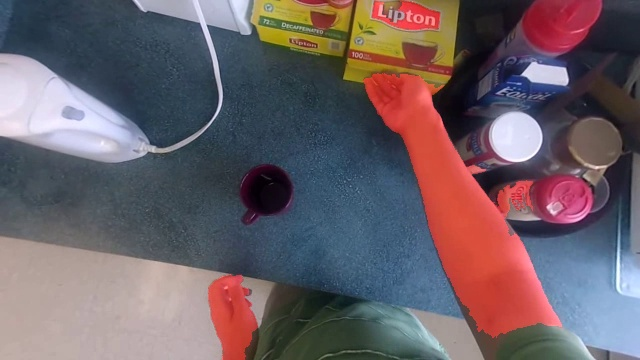
\includegraphics[width=.45\columnwidth]{./Figures/context-free2.jpg}
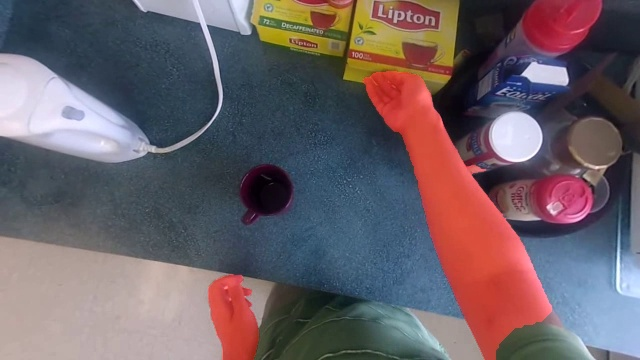
\includegraphics[width=.45\columnwidth]{./Figures/context-dependent2.jpg}
\caption{Comparison before (left image) and after (right image) Temporal smoothing.}
\label{fig:gesture_samples_time}
\end{figure}
Temporal smoothing aims to improve the foreground prediction of a pixel in a frame by a weighted combination of
its previous frames, since past frames should affect the results prediction for the current frame. This technique is inspired by \cite{liu08}.

The smoothing filter for a pixel $\mathbf{x}_{t}^{i}$ of a frame $t$  can thus be defined as follows:

\begin{multline}
P(\mathbf{x}_{t}^{i}=1) = \sum_{k = 0}^{\min(d,k)} w_{k} \bigl( P(\mathbf{x}_{t}^{i}=1|\mathbf{x}_{t-k}^{i}=1) \cdot P(\mathbf{x}_{t-k}^{i}=1|\mathbf{l_{t-k}},\mathbf{g_{t-k}})\, + P(\mathbf{x}_{t}^{i}=1|\mathbf{x}_{t-k}^{i}=0) \, \cdot \\
\cdot P(\mathbf{x}_{t-k}^{i}=0|\mathbf{l_{t-k}},\mathbf{g_{t-k}}) \bigr)
\end{multline}
where $P(\mathbf{x}_{t-k}^{i}=1|\mathbf{l_{t-k}},\mathbf{g_{t-k}})$ is the posterior probability
that a pixel in frame $t-k$ is marked as hand part and $d$ is a number of past frames used. This likelihood can be defined as the probability $P(\mathbf{s}|\mathbf{l_{t-k}},\mathbf{g_{t-k}})$, being
$\mathbf{x}_{t}^{i}$ part of $\mathbf{s}$. In the same way, $P(\mathbf{x}_{t-k}^{i}=0|\mathbf{l_{t-k}},\mathbf{g_{t-k}})$ is defined as the probability
$1-P(\mathbf{s}|\mathbf{l},\mathbf{g_{t-k}})$. 

While $P(\mathbf{x}_{t}^{i}=1|\mathbf{x}_{t-k}^{i}=1)$ and $P(\mathbf{x}_{t}^{i}=1|\mathbf{x}_{t-k}^{i}=0)$ are prior probabilities estimated
from the training set as follows:

\begin{equation}
P(\mathbf{x}_{t}^{i}=1|\mathbf{x}_{t-k}^{i}=1)=\frac{\#(\mathbf{x}_{t}^{i}=1,\mathbf{x}_{t-k}^{i}=1)}{\#(\mathbf{x}_{t-k}^{i}=1)}
\end{equation}


\begin{equation}
P(\mathbf{x}_{t}^{i}=1|\mathbf{x}_{t-k}^{i}=0)=\frac{\#(\mathbf{x}_{t}^{i}=1,\mathbf{x}_{t-k}^{i}=0)}{\#(\mathbf{x}_{t-k}^{i}=0)}
\end{equation}


where $\#(\mathbf{x}_{t-k}^{i}=1)$ and $\#(\mathbf{x}_{t-k}^{i}=0)$ are the number of times in which $\mathbf{x}_{t-k}$ belongs or not to
a hand region, respectively; $\#(\mathbf{x}_{t}^{i}=1,\mathbf{x}_{t-k}^{i}=1)$ is the number
of times that two pixels at the same location at frame $t$ and $t-k$ belong to a hand part; 
similarly, $\#(\mathbf{x}_{t}^{i}=1,\mathbf{x}_{t-k}^{i}=0)$
is the number of times that a pixel in frame $t$ belongs to
a hand part and pixel in the same position in frame $t-k$ does not belong
to a hand region. 

Based on our preliminary experiments we set $d$ equal to three.
Figure \ref{fig:gesture_samples_time} shows an example where temporal smoothing deletes blinking regions (i.e. the tea box brand and jar shadows on the right).


\subsection{Spatial consistency}
\begin{figure}[tb]
\centering
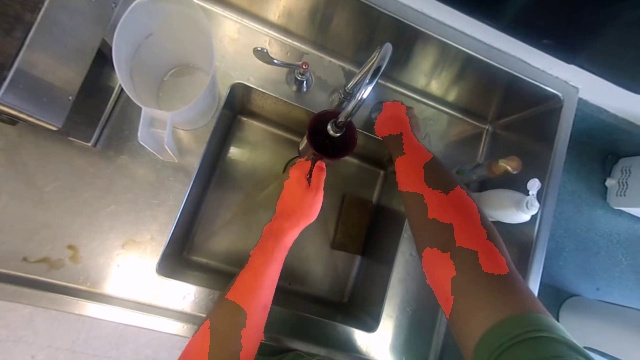
\includegraphics[width=.45\columnwidth]{./Figures/context-free1.jpg}
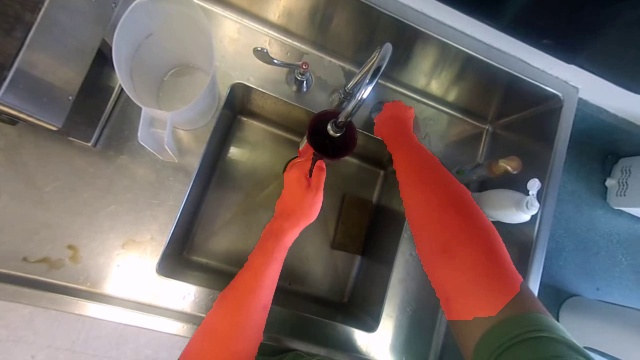
\includegraphics[width=.45\columnwidth]{./Figures/context-dependent1.jpg}
\caption{Comparison before (left image) and after (right image) Spatial Consistency.}
\label{fig:gesture_samples_space}
\end{figure}
Given pixels elaborated by the previous steps, we want to exploit spatial consistency to prune away small and isolated pixel groups that are unlikely to be part of hand regions and also aggregate bigger connected pixel groups. To this aim, we exploit the GrabCut algorithm \cite{rother04}, which essentially works as follows:

\begin{figure}[htbp]
	\centering
		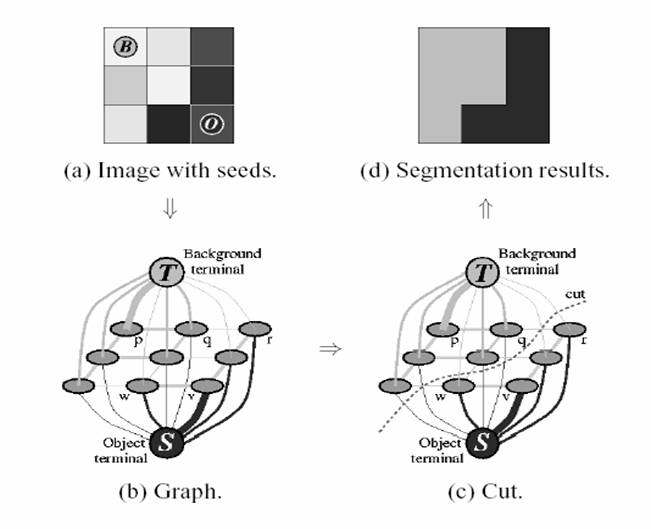
\includegraphics[width=.55\linewidth]{Figures/grabcut.jpg}
	\caption{The GrabCut algorithm.}
	\label{fig:GrabCut}
\end{figure}
 
\begin{enumerate}
\item It takes as input an initial trimap by of background, foreground and unknown pixels.
\item It creates an initial image segmentation, where all unknown
pixels are tentatively placed in the foreground class
and all known background pixels are placed in the background
class.
\item Gaussian Mixture Models (GMMs) are created for initial foreground
and background classes.
\item Each pixel in the foreground class is assigned to the most
likely Gaussian component in the foreground GMM. Similarly,
each pixel in the background is assigned to the most
likely background Gaussian component.
\item The GMMs are thrown away and new GMMs are learned from
the pixel sets created in the previous set.
\item A graph is built and Graph Cut is run to find a new tentative
foreground and background classification of pixels (Fig. \ref{fig:GrabCut}).
\item Steps 4-6 are repeated until the classification converges

\end{enumerate}

For every pixel $\mathbf{x}$, we extract its posterior probability $P(\mathbf{x}_{t}^{i})$ and use it as input for the GrabCut algorithm. Each pixel with $P(\mathbf{x}_{t}^{i}) \geq 0.5$ is marked as foreground, otherwise it's considered as part of background. After the segmentation step, we discard all the small isolated regions that have an area of less than 5\% of the frame and we keep only the three largest connected components.

In Figure \ref{fig:gesture_samples_space} an example with and without applying the Spatial Consistency method is depicted; notice this technique allows to better aggregate superpixels that are near the principal blob region.


\begin{figure*}[tb]
\centering
\subfigure[]{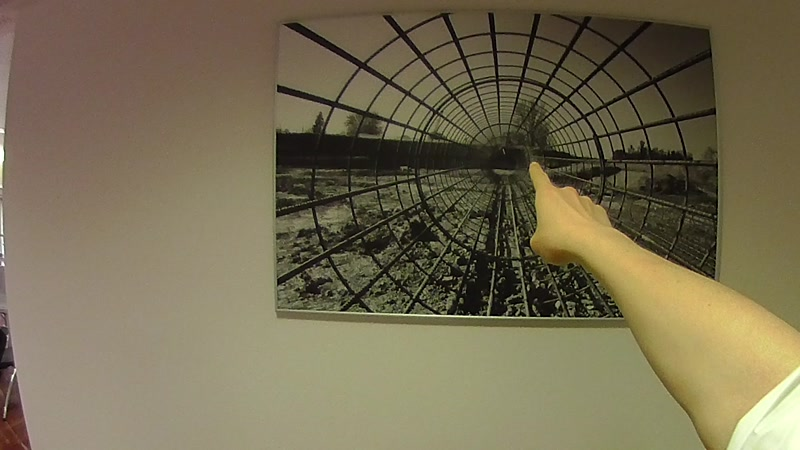
\includegraphics[width=.30\columnwidth]{./Figures/index_sample.jpg}}
\subfigure[]{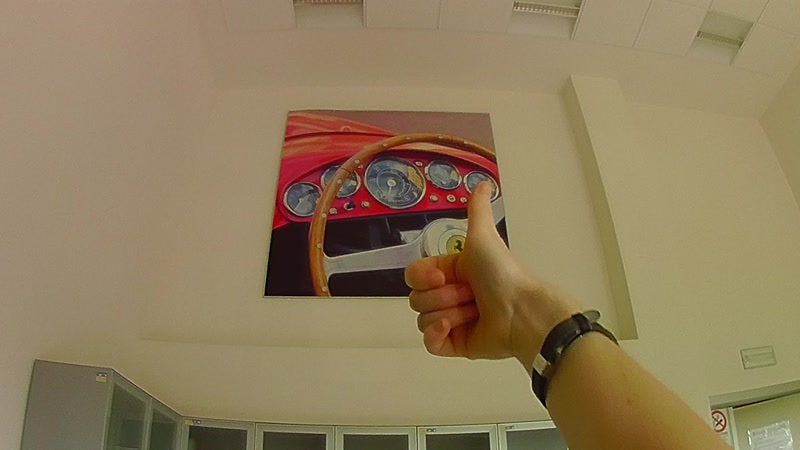
\includegraphics[width=.30\columnwidth]{./Figures/like_sample.jpg}}
\subfigure[]{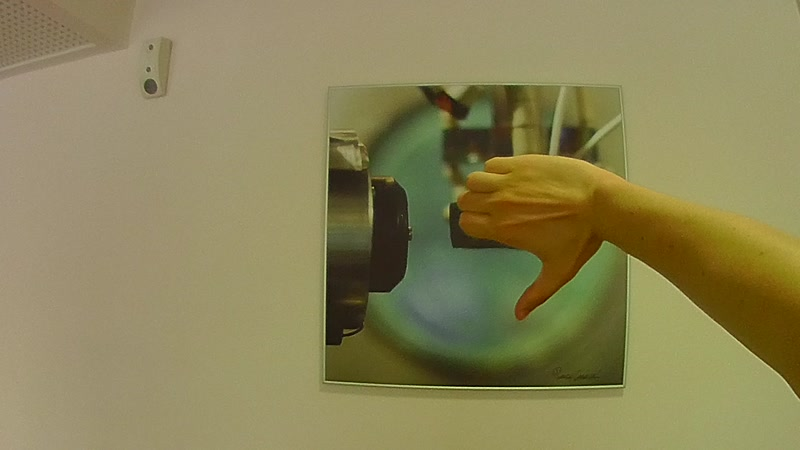
\includegraphics[width=.30\columnwidth]{./Figures/dislike_sample.jpg}}
\subfigure[]{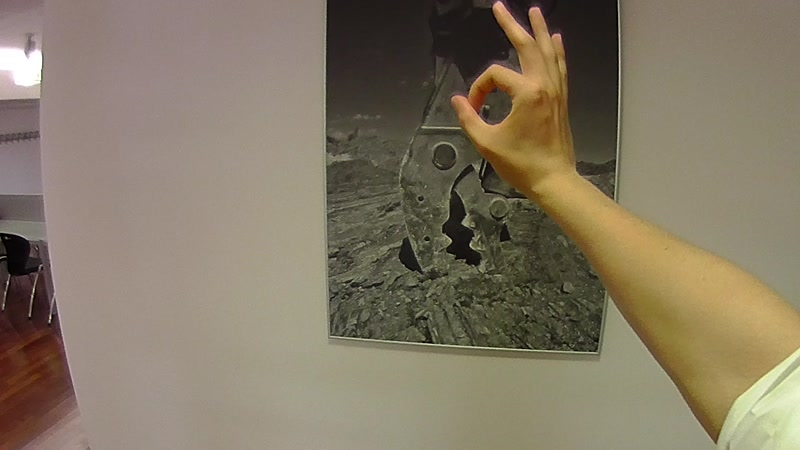
\includegraphics[width=.30\columnwidth]{./Figures/ok_sample.jpg}}
\subfigure[]{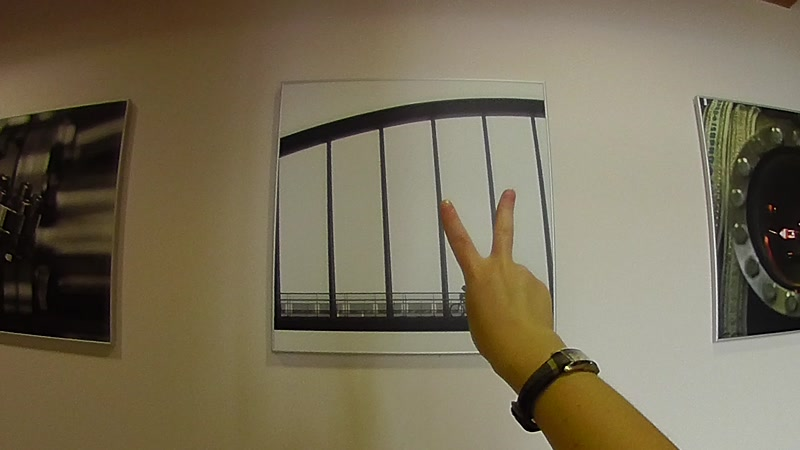
\includegraphics[width=.30\columnwidth]{./Figures/victory_sample.jpg}}
\caption{The EGO-HSGR dataset contains hands performing five gestures: a) point out; b) like; c) dislike; d) ok; e) victory.}
\label{fig:gesture_samples}
\end{figure*}

\section{Experimental results}
Having fully described our method, we now want to evaluate its performance on two datasets: EDSH and EGO-HSGR.
The recent publicly available EDSH dataset \cite{li13} consists in egocentric videos acquired to analyze performance of several hand detection methods. It consists of three videos (EDSH\_1, used as train video, and EDSH\_2 and EDSH\_{kitchen} used as test videos) that contain indoor and outdoor scenes with large variations of illumination, mild camera motion induced by walking and climbing stairs. All videos are recorded at a resolution of 720p and a speed of 30 fps. Also, the dataset includes segmentation masks of hands.    

We also generated a new dataset which contains 12 videos of indoor scenes (EGO-HSGR). Videos have been recorded with a Panasonic HX-A10 Wearable Camcorder (see \ref{panasonic}) at a resolution of $800 \times 450$ with a 25FPS in two different locations: a library and department's exhibition area.   

The aim of this dataset is to reproduce an environment similar to a museum for human and object interaction: paintings and posters are hung on the walls, true masterpieces or either its virtual images; the visitor walks and sometimes stops in front of an object of interest performing some gestures to interact with next generation wearable devices. We identify five different gestures that are used commonly: \textit{point out}, \textit{like}, \textit{dislike}, \textit{ok} and \textit{victory}. These can be associated to different action or used for record social experience. Fig. \ref{fig:gesture_samples} shows some frame examples. 

To evaluate performance of our pixel-level hand detector a subset of six videos are used (three for training and two for testing). Segmentation masks are provided every 25 frames for a total of 700 annotations. 
The F-score (harmonic mean of the precision and recall rate) is used to quantity hand detection performance.
%(we denote these videos as BB\_L1 and BB\_L2), a corridor of a faculty (BB\_F1 and BB\_F2) and a department (BB\_D1 and BB\_D2).

In the following subsections, we are going to evaluate every single aspect of our method: the performance of the features, and of the proposed techniques: temporal consistency, spatial coherence and illumination invariance. We will also compare our approach to existing methods.
    
 \begin{table}
 \centering
 \begin{tabular}{|l|c|c|}
 \hline
 \textbf{Features} 	& \textbf{EDSH\_2} & \textbf{EDSH\_{kitchen}}	\\ \hline\hline
 HSV	& 0.752 & 0.801		\\ \hline
 + LAB	& 0.754	&	0.808 \\ \hline
 + LAB hist.	& 0.755 & 0.823			\\ \hline  
 + HSV hist. & 0.755 & 0.823			\\ \hline  
 + Grad hist. & 0.758	&	0.828	\\ \hline  
 + Gabor & 	\textbf{0.761}	& \textbf{0.829} \\ \hline  
 \end{tabular}
 \caption{Performance by incrementally adding new features.}\label{tab:localfeatures}
 \end{table}

\subsection{Features performance}

First, we examine the effectiveness of our features to discriminate between hand and non-hand superpixels. 
Table \ref{tab:localfeatures} shows performance in terms of F-measure on EDSH dataset with different feature combinations: firstly we describe each superpixel with mean and covariance matrix of its pixel values in HSV colour space, then we do the same using LAB colour space and we add colour histograms. Lastly, we include a histogram of gradients and Gabor feature.
In order to analyze how visual features impact on the performance, in this experiment we do not include the temporal and spatial context information by using a single random forest classifier.     
Note that although colour information plays a fundamental role for hand detection, some ambiguities between hands and other similar coloured object still remain; these can be reduced by adding features based on gradient histograms. In fact, the usage of the full descriptor slightly improves the performance.      

\begin{table}
 \centering
 \begin{tabular}{|l|c|c|}
 \hline
 \textbf{Features} 	& \textbf{EDSH\_2} & \textbf{EDSH\_{kitchen}}	\\ \hline\hline
 II	& 0.789 & 	0.831		\\ \hline
 II + TS	& 0.791	&	0.834 \\ \hline
 II + TS + SC &	\textbf{0.852} &	\textbf{0.901}	\\ \hline  
 \end{tabular}
 \caption{Performance comparison considering Illumination Invariance (II), Time Smoothing (TS) and Spatial Consistency (SC).}\label{tab:context}
\end{table}


\subsection{Temporal Smoothing and Spatial Consistency}
In this experiment we validate the proposed techniques that take into account illumination variations, time dependence and spatial consistency.
Table \ref{tab:context} shows the F-measure scores obtained on EDSH dataset incrementally adding Illumination Invariance (II), Time Smoothing (TS) and Spatial Consistency (SC). 
Note that there is a significant improvement in performance when all these three techniques are applied together.   
In particular, illumination invariance substantially increases the performance with respect to results obtained using only visual features and a single random forest classifier, while the improvement introduced by temporal smoothing is less pronounced. The main contribution is given by Spatial Consistency, that prunes away small and isolated pixel groups and merge spatially nearby regions, increasing the F-measure score of about six percentage points.
The proposed technique is also tested in our EGO-HSGR dataset obtaining an F-measure score of $0.908$ and $0.865$ for the EGO-HSGR\_{4} and EGO-HSGR\_{5} videos.        


\begin{table}
 \centering
 \begin{tabular}{|l|c|c|}
 \hline
  	& \textbf{EDSH\_2}	& \textbf{EDSH\_{kitchen}} \\ \hline\hline
Video stabilization  \cite{hayman03} 	& 0.211 & 0.213		\\ \hline
Single pixel colour \cite{jones99}	& 0.708 &	0.787	\\ \hline  
Collection of random forest \cite{li13} & 0.835 & 0.840		\\ \hline  
\textbf{Our method} & \textbf{0.852} &	\textbf{0.901}	\\ \hline 
\end{tabular}
\caption{Hand segmentation comparison with the state-of-the-art.}\label{tab:comparision_hand}
\end{table}



\subsection{Comparison to related methods}

In Table \ref{tab:comparision_hand} we compare our results to several approaches on EDSH dataset: a single-pixel colour approach inspired by \cite{jones99}, a video stabilization approach based on background modeling using affine alignment of image frames inspired by
\cite{hayman03} and the approach based on random forest, by Li \etal \cite{li13}. 
The single-pixel approach is a random regressor trained only using single-pixel LAB colour values. 
The background modeling approach aligns sequences of 15 frames estimating their mutual affine transformations; pixels with high variance are considered to be foreground hand regions. 
As can be seen, although the single-pixel approach is conceptually simple, is still quite effective. In addition, we observe that the low performance of the video stabilization approach is due to large ego-motion because the camera is worn by the user.     
The method recently proposed by \cite{li13} is more similar to our approach, but the use of superpixels, the selection of a new set of local features and the introduction of temporal and spatial consistency allow us to outperforms that results.

\medskip
We have addressed one of the main issues involved in hand gesture recognition: hand segmentation. The proposed algorithm will be exploited in the next chapter, where our gesture recognition approach will be introduced and fully described.


% Chapter 1

\chapter{Gesture recognition in the cultural heritage scenario}

\lhead{Chapter 4. \emph{Hand gesture recognition}} % This is for the header on each page - perhaps a shortened title

%----------------------------------------------------------------------------------------
Having presented our hand segmentation approach, we move a step forward and introduce a more complex problem: detecting static and dynamic hand gestures. As we said in the introductory chapter, the target scenario of our research is the cultural heritage domain. In fact, our goal is to deploy new gesture-based human machine interfaces to enhance museum experience.

\section{Motivation}
In recent years the interest in cultural heritage has reborn, and the cultural market is becoming a cornerstone in many national economic strategies. In the United States, a recent report of the Office of Travel and Tourism Industries claims that 51\% of the 40 million Americans traveling abroad visit historical places; almost one third visit cultural heritage sites; and one quarter go to an art gallery or museum \cite{tourismintelligence}. The same interest is found in Europe, where the importance of the cultural sector is widely acknowledged, South Asia and North Africa. The latest annual research from World Travel and Tourism Council shows that travel and tourism's total contribution to total GDP grew by 3.0\% in 2013, faster than overall economic growth for the third consecutive year \cite{econotravel}.

Consequently, to deal with an increasing percentage of ``digital native'' tourists, a big effort is under way to propose new interfaces for interacting with the cultural heritage.
 In this direction goes the solution ``SmartMuseum'' proposed by Kuusik \etal \cite{kuusik2009smartmuseum}: by the means of PDAs and RFIDs, a visitor can gather information about what the museum displays, building a customized visit based on his or her interests inserted, prior to the visit, on their website. This project brought an interesting novelty when first released, but it has some limitations. First, being tied to RFIDs does not allow reconfiguring the museum without rethinking the entire structure of the exhibition. Furthermore, researches demonstrated how the use of mobile devices on the long term decreases the quality of the visit due to their users paying more attention to the tool rather than to the work of art itself.

In 2007 Kuflik \etal \cite{kuflik2011visitor} proposed a system to customize visitors experiences in museums using software capable of learning their interests based on the answers to a questionnaire that they compiled before the visit. Similarly to SmartMuseum, one of the main shortcomings of this system is the need to stop the visitor and force him into doing something that he/she might not be willing to do.
An interesting attempt to user profiling with wearable sensors was the Museum Wearable \cite{sparacino2002museum}, a wearable computer which orchestrates an audiovisual narration as a function of the visitors' interests gathered from his/her physical path in the museum. However this prototype does not use any computer vision algorithm for understanding the surrounding environment. For instance the estimation of the visitor location is based again on infrared sensors distributed in the museum space.

Museums and cultural sites still lack of an instrument that provides entertainment, instructions and visit customization in an effective natural way. Too often visitors struggle to find the description of the artwork they are looking at and when they finds it, its detail level could be too high or too low for their interests. Moreover, frequently the organization of the exhibition does not reflect the visitors' interests leading them to a pre-ordered path which cultural depth could not be appropriate.

To overcome these limitations, we try to enhance visitors' experiences using ego-vision. Ego-vision features glass-mounted wearable cameras able to see what the visitor sees and perceiving the surrounding environment as he does. Our goal is to develop a wearable vision device for museum environments, able to replace the traditional self-service guides and overcoming their limitations and allowing for a more interactive museum experience to all visitors. The aim of our device is to stimulate the visitors to interact with the artwork, reinforcing their real experience, by letting visitors to replicate the gestures (e.g. point out to the part of the painting they're interested in) and behaviors that they would use to ask a guide something about the artwork (see Fig. \ref{sample} for some samples of the recognized gestures).

In this chapter, we provide algorithms that perform gesture analysis to recognize user interaction with artworks. We also propose to use scalable and distributed wearable devices capable of communicating with each other and with a central server. In particular the connection with the central server allows our wearable devices to grab gestures of past visitors for improving gesture analysis accuracy.

The proposed gesture recognition algorithm is compared to the current state of the art on benchmark datasets showing superior performance, and is tested in real and virtual museum environments. We further demonstrate that our gesture recognition approach can achieve acceptable accuracy results even with a few training samples performed by the visitor, and can benefit from distributed training in which gestures performed by other visitors are exploited.


\section{Proposed Method}
To our knowledge, the study of gesture recognition in the ego-centric paradigm has not yet been addressed. Even though not related to ego-vision domain, several approaches to gesture and human action recognition have been proposed. Sanin \etal \cite{sanin2013spatio} developed a new and more effective spatio-temporal covariance descriptor to classify gestures in conjunction with a boost classifier. Lui \etal \cite{lui2010action, lui2011tangent} used tensors and tangent bundle on Grassmann manifolds to classify human actions and hand gestures. Kim \etal \cite{kim2009canonical} extended Canonical Correlation Analysis to measure video-to-video similarity to represent and detect actions in video. However, all these approaches are not appropriate for the ego-centric perspective, as they do not take into account any of the specific characteristics of this domain, such as fast camera motion and background cluttering.
\begin{figure}
\centering
\subfigure{
                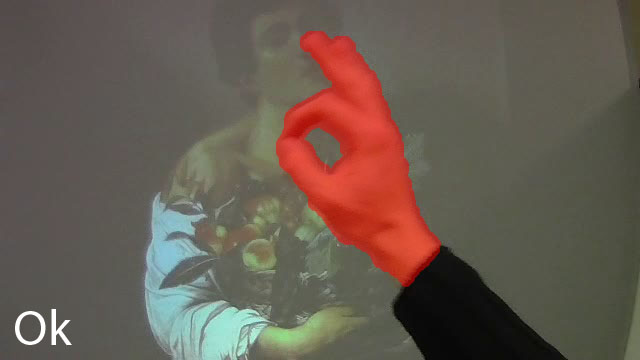
\includegraphics[width=0.23\textwidth]{Figures/ok_7141_7164_text16.jpg}
                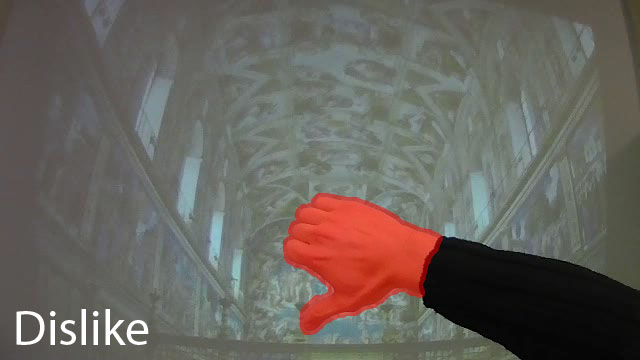
\includegraphics[width=0.23\textwidth]{Figures/dislike_3941_3969_text16.jpg}
} \\
\subfigure{
	    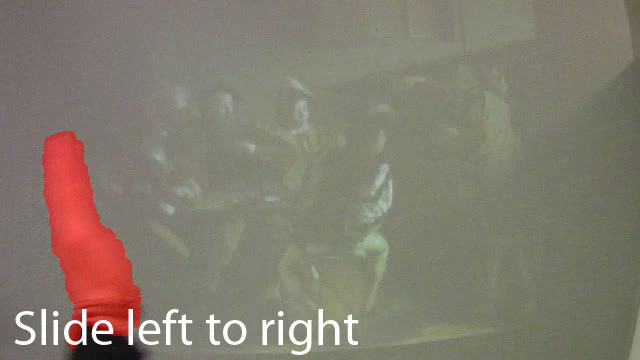
\includegraphics[width=0.23\textwidth]{Figures/slide_2_7438_7451_text5.jpg}
                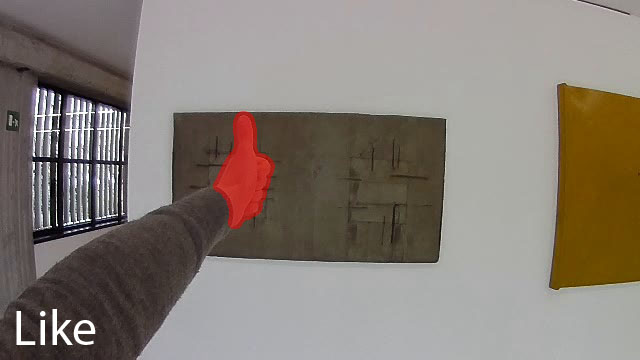
\includegraphics[width=0.23\textwidth]{Figures/like_7038_7080_text23.jpg}
} \\
\subfigure{
                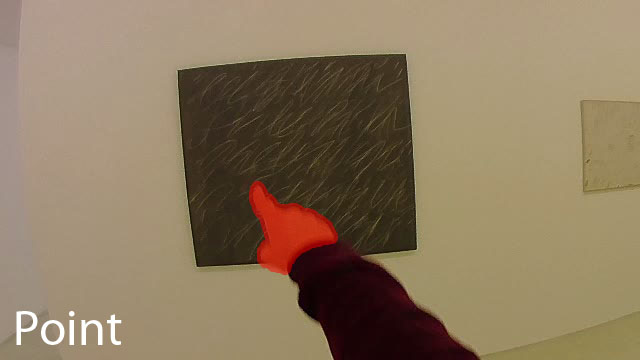
\includegraphics[width=0.23\textwidth]{Figures/point_15476_15505_text5.jpg}
                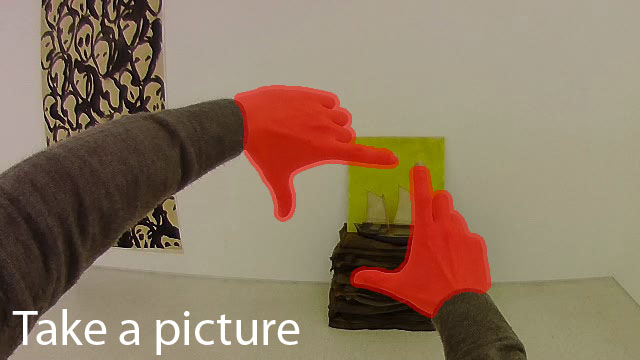
\includegraphics[width=0.23\textwidth]{Figures/take_a_picture_18622_18673_text37.jpg}
} \\
\caption{Results from the proposed hand segmentation and gesture recognition algorithms. Hand segmentation results are highlighted in red and detected gestures are reported in the bottom part of each frame.}
\label{sample}
\end{figure}

\begin{figure}
\centering
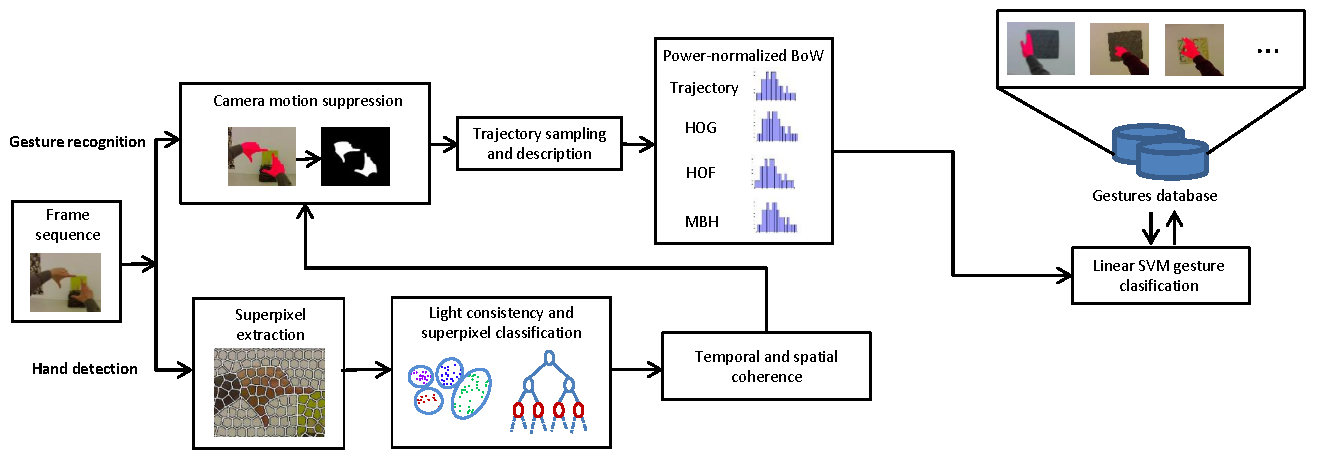
\includegraphics[width=\linewidth]{Figures/schema.pdf}
\caption{Outline of the proposed Gesture Recognition method.}
\label{schema}
\end{figure}
Gesture recognition systems should recognize both static and dynamic hand movements. Therefore, we propose to describe each gesture as a collection of dense trajectories extracted around hand regions. Feature points are sampled inside and around the user's hands and tracked during the gesture; then several descriptors are computed inside a spatio-temporal volume aligned with each trajectory, in order to capture its shape, appearance and movement at each frame. 
These descriptors are coded,  using the Bag of Words approach and power normalization, in order to obtain the final feature vectors, which are then classified using a linear SVM classifier. A summary of our approach is presented in Figure \ref{schema}.

In the next subsections we will introduce the main components of our approach: camera motion suppression, trajectory sampling and description, the power normalized Bag of Words and the final classification. We will also explain how these steps exploit the hand segmentation approach we have presented in the previous chapter.

\subsection{Feature points sampling}
We start by describing how we densely sample feature points for generating trajectories. To this aim, we consider a grid spaced by $W$ pixels. Sampling is carried out on each
spatial scale separately. This guarantees that feature points equally cover all spatial
positions and scales. Experimental results showed that a sampling step size of $W = 5$ pixels is dense
enough to give good results over all datasets. There are at most 8 spatial scales in total, depending on the
resolution of the video. The spatial scale increases by a factor of $1/\sqrt{2}$.
Our goal is to track all these sampled points through the video. However, in homogeneous image
areas without any structure, it is impossible to track any point. We remove points in these areas. Here, we
use the criterion that the points are removed if the eigenvalues of the auto-correlation
matrix are very small. We set a threshold $T$ on the eigenvalues for each frame $I$ as
\begin{equation}
T = 0.001 \times \max_{i\in I} \min(\lambda_i^1, \lambda_i^2)
\end{equation}

where $(\lambda_i^1, \lambda_i^2)$ are the eigenvalues of point $i$ in the image $I$. Experimental results showed that a value
of 0.001 represents a good compromise between saliency and density of the sampled points.

\subsection{Camera motion suppression}
A key step in our approach is to remove camera motion. To this end, the homography between two consecutive frames is estimated running the RANSAC algorithm on features points sampled as described. 

An homography (or \textit{projective transformation}) is defined by the following equation, where $x_1$ and $x_2$ are 2-d points expressed in homogeneous coordinates:
$$
x_1 = \left[\begin{array}{c c c}
 h_{11} & h_{12} & h_{13} \\
 h_{21} & h_{22} & h_{23} \\
 h_{31} & h_{32} & h_{33}
 \end{array}\right] x_2
$$
and, because two homography matrices that differ for a scale are equivalent, this matrix has only 8 degrees of freedom. RANSAC is accomplished to produce a good homography with the following steps:
\begin{enumerate}
\item Randomly selecting a subset of feature points
\item Fitting an homography to the selected subset
\item Determining the number of outliers
\item Repeating steps 1-3 for a prescribed number of iterations, and select the iteration with the minimum amount of outliers
\end{enumerate}

This would be the standard way to fit an homography between two frames. However, in first-person camera views hands movement is not consistent with camera motion and this generates wrong matches between the two frames. For this reason we introduce a segmentation mask that disregards feature matches belonging to hands. In fact, without the hand segmentation mask, many feature points from the user's hands would become inliers, degrading the homography estimation. As a consequence, the trajectories extracted from the video would be incorrect. Instead, computing an homography using feature points from non-hand regions allows us remove all the camera movements.

\subsection{Trajectory Sampling and description}
Having removed camera motion between two adjacent frames, trajectories can be extracted. The second frame is warped with the estimated homography, the optical flow between the first and the second frame is computed, and then feature points around the hands of the user are sampled and tracked following what \cite{wang:2011:inria-00583818:1} does for human action recognition.

Feature points are tracked on each spatial scale separately. For each frame $I_t$, its dense optical flow field
$\omega_t = (u_t, v_t)$ is computed w.r.t. the next frame $I_{t+1}$, where $u_t$ and $v_t$ are the horizontal and vertical
components of the optical flow. Given a point $P_t = (x_t, y_t)$ in frame $I_t$, its tracked position in frame $I_{t+1}$
is smoothed by applying a median filter on $\omega_t$:
\begin{equation}
P_{t+1} = (x_{t+1}, y_{t+1}) = (x_t, y_t) + (M * \omega_t)
\end{equation}
where $M$ is the median filtering kernel. The size of the median filter kernel $M$ is $3 \times 3$ pixels. As the
median filter is more robust to outliers than bilinear interpolation, it improves trajectories
for points at motion boundaries that would otherwise be smoothed out.
Once the dense optical flow field is computed, points can be tracked very densely without additional
cost. Another advantage of the dense optical flow is the smoothness constraints which allow relatively
robust tracking of fast and irregular motion patterns. To extract dense optical flow fields, we
use Farneback's algorithm \cite{farneback2003two} which embeds a translation motion model between neighborhoods of two consecutive
frames. Polynomial expansion is employed to approximate pixel intensities in the neighborhood.

Points of subsequent frames are concatenated to form trajectories: $(P_t,  P_{t+1}, P_{t+2}, ...))$. As trajectories
tend to drift from their initial locations during the tracking process, we limit their length to $L$ frames
in order to overcome this problem (based on our preliminary tests, we set $L=30$). For each frame, if no tracked point is found
in a $W \times W$ neighborhood, a new point is sampled and added to the tracking process so that a dense coverage
of trajectories is ensured.

As static trajectories do not contain motion information, we prune them in a post-processing stage.
Trajectories with sudden large displacements, most likely to be erroneous, are also removed. Such trajectories
are detected, if the displacement vector between two consecutive frames is larger than 70\% of the
overall displacement of the trajectory.

Furthermore, in contrast to what \cite{wang:2011:inria-00583818:1} does, trajectories are restricted to lie inside and around the user's hands: at each frame the hand mask is dilated, and all the feature points outside the computed mask are discarded.


Then, the spatio-temporal volume aligned with each trajectory is considered, and Trajectory descriptor, HOG, HOF and MBH are computed around it. The trajectory descriptors encodes local motion patterns. Given a trajectory of length $L$, we describe its
shape by a sequence $(\Delta P_t, ..., \Delta P_{t+L-1})$ of displacement vectors $\Delta P_t = (P_{t+1}- P_t) = (x_{t+1} -
xt, y_{t+1}- y_t)$. The resulting vector is normalized by the sum of displacement vector magnitudes:
\begin{equation}
T = \frac{(\Delta P_t, .., \Delta P_{t+L-1})}{\sum_{j=t}^{t+L-1} \| \Delta P_j \|}
\end{equation}
As we use trajectories with a fixed length of $L = 30$ frames, we obtain a 60 dimensional descriptor.

Besides the trajectory shape information, we also design descriptors to embed appearance and motion
information. We compute
descriptors within a space-time volume aligned with a trajectory to encode the motion information. The size of the volume is $N \times N$ pixels and $L$ frames long. To embed structure information, the volume is subdivided into a spatio-temporal grid of size $n_\sigma \times n_\sigma \times n_\tau$. We compute a descriptor (e.g.,
HOG, HOF or MBH) in each cell of the spatio-temporal grid, and the final descriptor is a concatenation
of these descriptors. The default parameters for our experiments are $N = 32$, $n_\sigma = 2$, $n_\tau = 3$.

As we have already said in Chapter \ref{chpt2}, HOG focuses on static appearance information, whereas HOF captures the
local motion information. We compute the HOG and HOF descriptors along the dense trajectories. For both HOG and HOF,
orientations are quantized into 8 bins with full orientation and magnitudes are used for weighting. An
additional zero bin is added for HOF (i.e., in total 9 bins). It accounts for pixels whose optical flow
magnitudes are lower than a threshold. Both descriptors are normalized with their $L_2$ norm. The final
descriptor size is 96 for HOG (i.e., $2\times 2\times 3\times 8$) and 108 for HOF (i.e., $2\times 2 \times 3 \times 9$).

The motion boundary histogram (MBH) descriptor computes derivatives separately for the horizontal and vertical components of the optical flow. The descriptor encodes the relative motion between pixels, and since MBH represents
the gradient of the optical flow, locally constant camera motion is removed and information about changes
in the flow field (i.e., motion boundaries) is kept. MBH is more robust to camera motion than optical flow,
and thus more discriminative.
We employ MBH s motion descriptor for trajectories. The MBH descriptor separates
optical flow $\omega = (u, v)$ into its horizontal and vertical components. Spatial derivatives are computed
for each of them and orientation information is quantized into histograms. The magnitude is used for
weighting. We obtain a 8-bin histogram for each component (i.e., MBHx and MBHy). Both histogram
vectors are normalized separately with their $L_2$ norm. The dimension is 96 (i.e., $2 \times 2 \times 3 \times 8$) for both
MBHx and MBHy.
For both HOF and MBH descriptor computation, we reuse the dense optical flow that is already
computed to extract dense trajectories.

While HOF and MBH are averaged on five consecutive frames, a single HOG descriptor is computed for each frame. In this way we can better describe how the hand pose changes in time. After this step, we get a variable number of trajectories for each gesture. In order to obtain a fixed size descriptor, the Bag of Words approach is exploited: we train four separate codebooks, one for each descriptor. Each codebook contains 500 visual words and is obtained running the $k$-means algorithm in the feature space. 

Since BoW histograms in our domain tend to be sparse, they are power normalized to unsparsify the representation, while still allowing for linear classification. To perform power-normalization \cite{perronnin2010improving}, the following function is applied to each bin $h_i$:
\begin{equation}
f(h_i) = \textrm{sign} (h_i) \cdot |h_i|^{\frac{1}{2}}
\end{equation}

We have also observed that power-normalization greatly improves the final accuracy. The feature vector is then obtained by the concatenation of its four power-normalized histograms. Eventually, gestures are recognized using a linear SVM 1-vs-1 classifier. SVM 1-vs-all and SVM Multiclass classifiers were also tested.

\section{Experimental Results}

We now evaluate the performance of the proposed approach. To compare the performance of our gesture recognition algorithm with existing approaches, we test it on the Cambridge-Gesture database \cite{kim2007tensor}, which includes nine hand gesture types performed on a table, under different illumination conditions. To better investigate the effectiveness of the proposed approach in videos taken from the ego-centric perspective and in a museum setting, we also propose two far more realistic and challenging dataset which contains seven gesture classes, performed by five subjects in an interactive exhibition room which functions as a virtual museum and in a real museum. 

The Cambridge Hand Gesture dataset contains 900 sequences of nine hand gesture classes. Although this dataset does not contain ego-vision videos it is useful to compare our results to recent gesture recognition techniques. In particular, each sequence is recorded with a fixed camera, placed over one hand, and hands perform leftward and rightward movements on a table, with different poses. The whole dataset is divided in five sets, each of them containing image sequences taken under different illumination conditions. The common test protocol, proposed in \cite{kim2007tensor}, requires to use the set with normal illumination for training and the remaining sets for testing, thus we use the sequences taken in normal illumination to generate the BoW codebooks and to train the SVM classifier. Then, we perform the test using the remaining sequences.   

Table \ref{cambridge} shows the recognition rates obtained with our gesture recognition approach, compared with the ones of tensor canonical correlation analysis (TCCA) \cite{kim2009canonical}, product manifolds (PM) \cite{lui2010action}, tangent bundles (TB) \cite{lui2011tangent} and spatio-temporal covariance descriptors (Cov3D) \cite{sanin2013spatio}. Results show that proposed method outperforms the existing state-of-the-art approaches.


\begin{table}
\begin{center}
\begin{tabular}{|l|c|c|c|c|c|}
\hline
\textbf{Method}					& \textbf{Set1}		& \textbf{Set2}		& \textbf{Set3}		& \textbf{Set4}	 	& \textbf{Overal}l \\
\hline
\hline
TCCA \cite{kim2009canonical}		& 0.81		& 0.81		& 0.78		& 0.86		& 0.82 \\
\hline
PM \cite{lui2010action}			& 0.89		& 0.86		& 0.89		& 0.87		& 0.88  \\
\hline
TB \cite{lui2011tangent}			& \textbf{0.93}	& 0.88		& 0.90		& 0.91		& 0.91 \\
\hline
Cov3D \cite{sanin2013spatio}		& 0.92		&\textbf{0.94}	& 0.94		& 0.93		& 0.93 \\
\hline
\textbf{Our method}			& 0.92		& 0.93		& \textbf{0.97}	& \textbf{0.95}	& \textbf{0.94} \\
\hline
\end{tabular}
\end{center}
\caption{Recognition rates on the Cambridge dataset.}
\label{cambridge}
\end{table}


\begin{figure}
\centering
\subfigure[\textit{Like} gesture in the \textit{museum} setting]{
  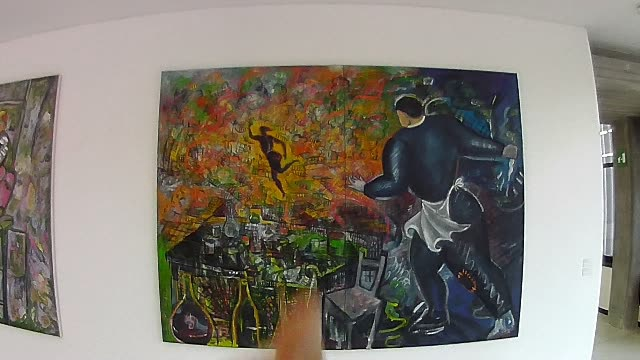
\includegraphics[width=0.2\linewidth]{Figures/like_16695_16718_all1.jpg}
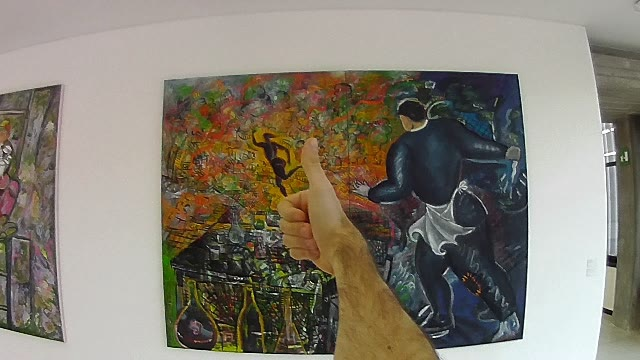
\includegraphics[width=0.2\linewidth]{Figures/like_16695_16718_all14.jpg}
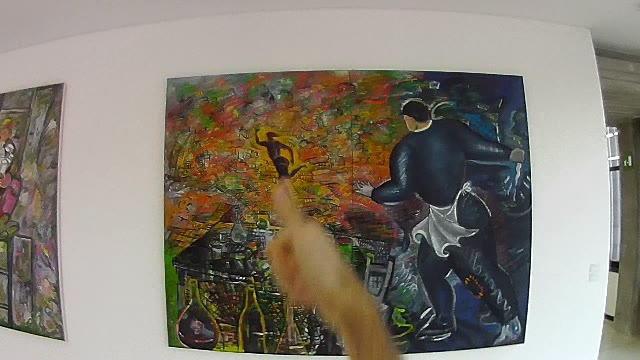
\includegraphics[width=0.2\linewidth]{Figures/like_16695_16718_all21.jpg}
}\\
\subfigure[\textit{Dislike} gesture]{
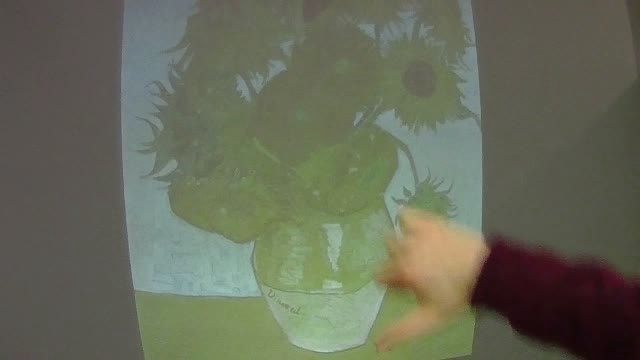
\includegraphics[width=0.2\linewidth]{Figures/dislike_10962_11000_all3.jpg}
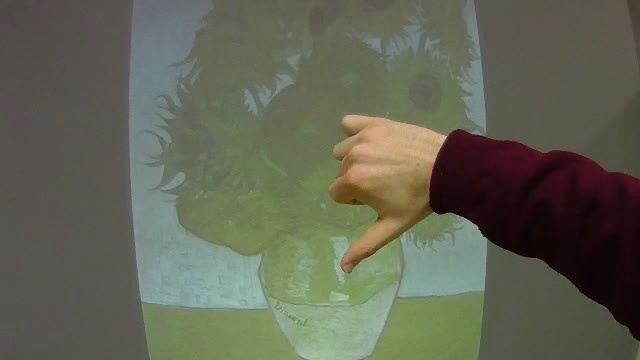
\includegraphics[width=0.2\linewidth]{Figures/dislike_10962_11000_all23.jpg}
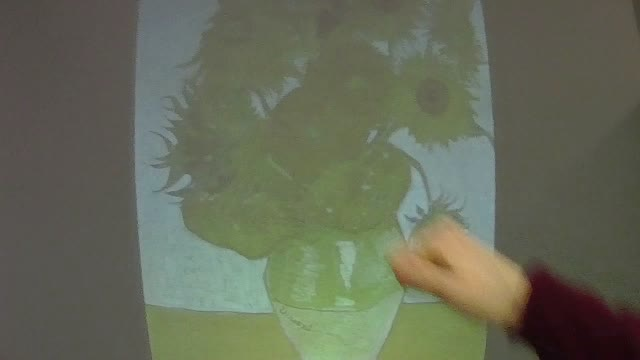
\includegraphics[width=0.2\linewidth]{Figures/dislike_10962_11000_all35.jpg}
}\\
\subfigure[\textit{Ok} gesture in the \textit{museum} setting, in low light]{
  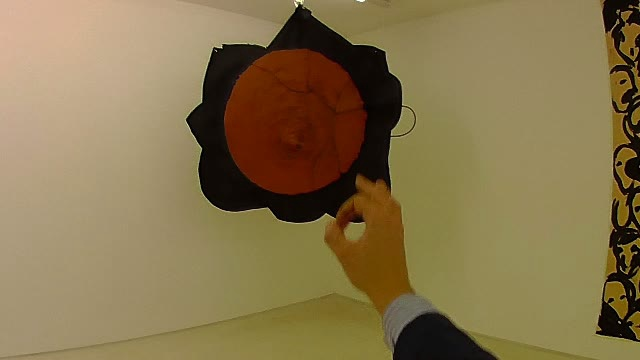
\includegraphics[width=0.2\linewidth]{Figures/ok_2696_2735_all5.jpg}
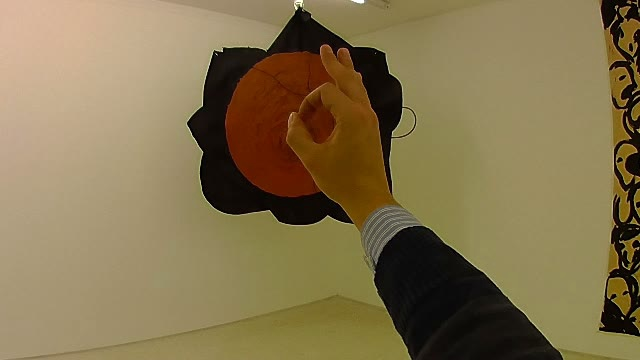
\includegraphics[width=0.2\linewidth]{Figures/ok_2696_2735_all23.jpg}
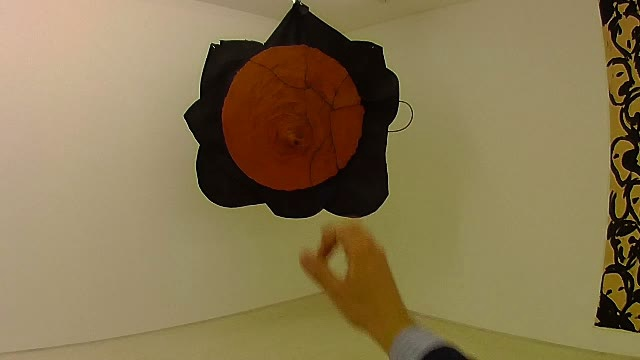
\includegraphics[width=0.2\linewidth]{Figures/ok_2696_2735_all36.jpg}
}\\
\subfigure[\textit{Point} gesture]{
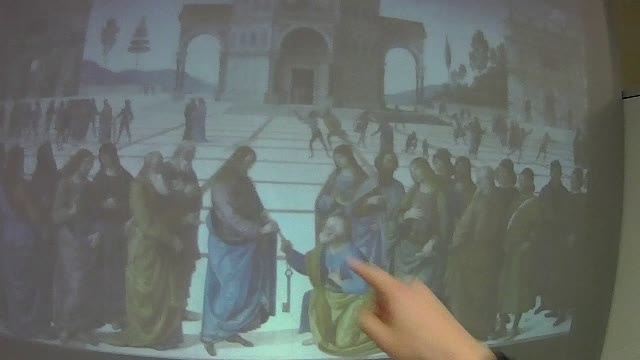
\includegraphics[width=0.2\linewidth]{Figures/point_4624_4654_all3.jpg}
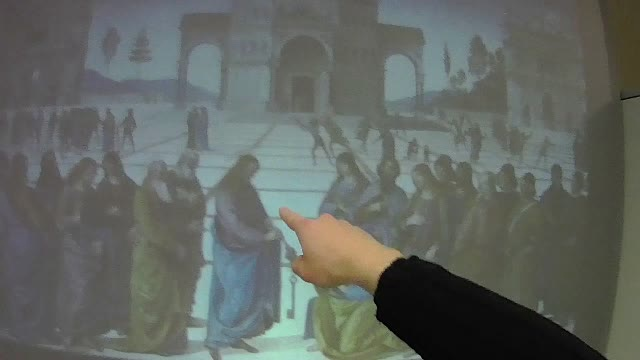
\includegraphics[width=0.2\linewidth]{Figures/point_4624_4654_all8.jpg}
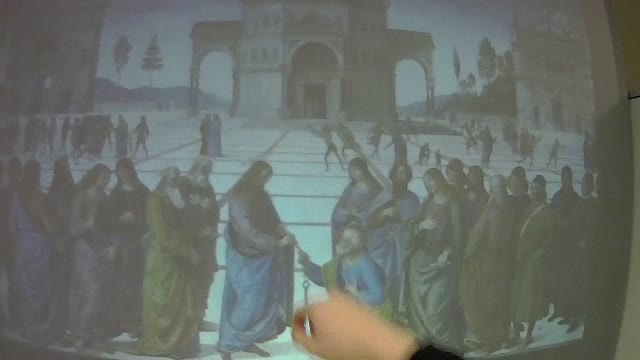
\includegraphics[width=0.2\linewidth]{Figures/point_4624_4654_all28.jpg}
}\\
\subfigure[\textit{Slide right to left} gesture in the \textit{museum} setting, while another visitor walks in]{
  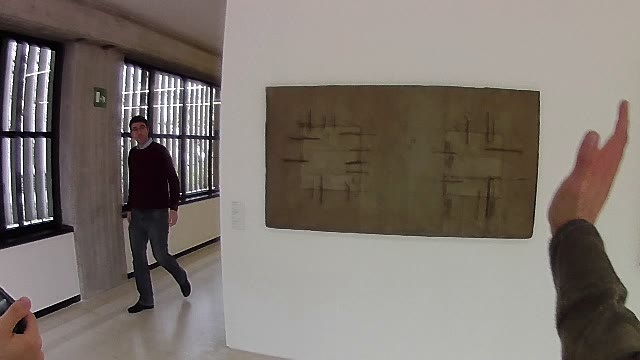
\includegraphics[width=0.2\linewidth]{Figures/slide_2_7348_7383_all12.jpg}
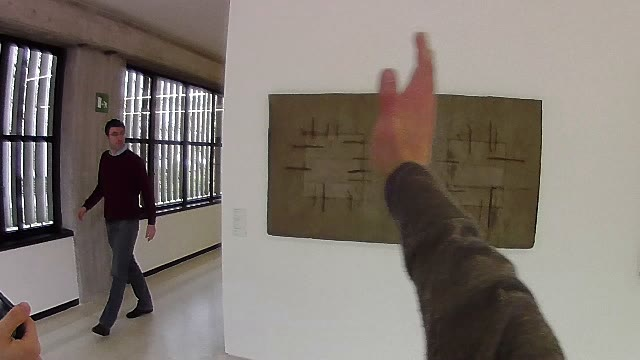
\includegraphics[width=0.2\linewidth]{Figures/slide_2_7348_7383_all20.jpg}
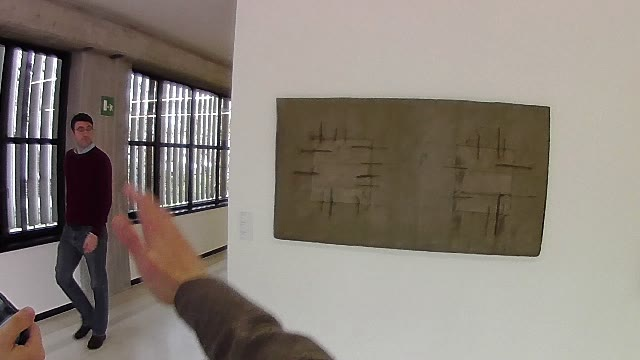
\includegraphics[width=0.2\linewidth]{Figures/slide_2_7348_7383_all30.jpg}
}\\
\subfigure[\textit{Slide left to right} gesture in the \textit{demo room} setting performed by user 3]{
  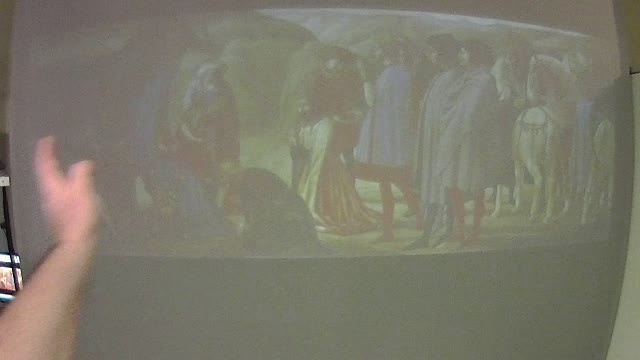
\includegraphics[width=0.2\linewidth]{Figures/slide_2_2030_2058_all7.jpg}
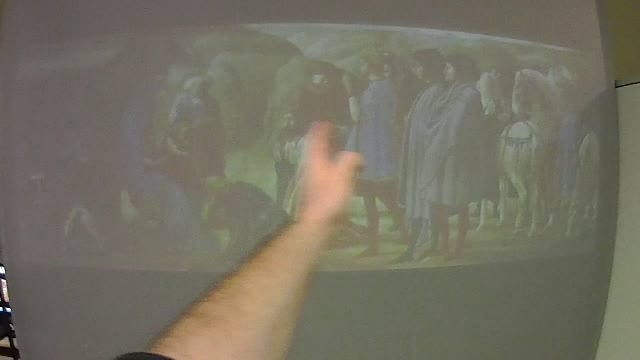
\includegraphics[width=0.2\linewidth]{Figures/slide_2_2030_2058_all14.jpg}
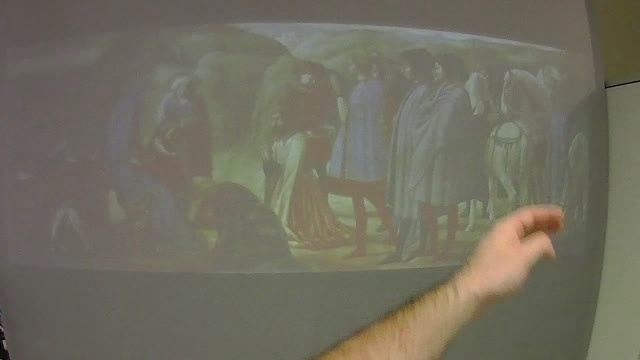
\includegraphics[width=0.2\linewidth]{Figures/slide_2_2030_2058_all23.jpg}
}\\
\subfigure[\textit{Take a picture} gesture in the \textit{demo room} setting]{
  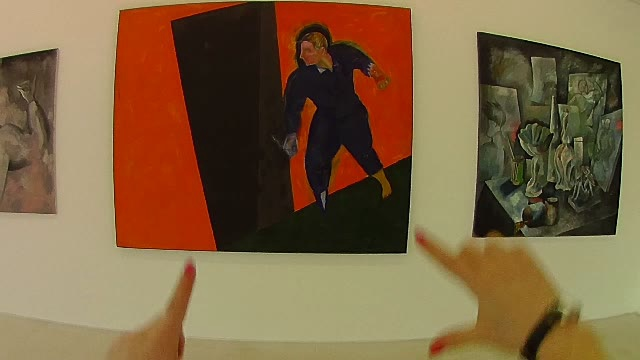
\includegraphics[width=0.2\linewidth]{Figures/take_a_picture_23956_24002_all2.jpg}
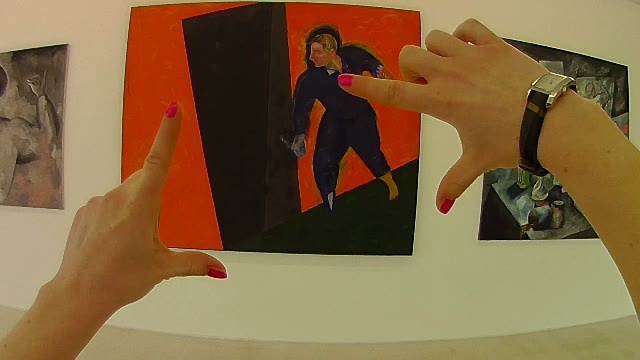
\includegraphics[width=0.2\linewidth]{Figures/take_a_picture_23956_24002_all25.jpg}
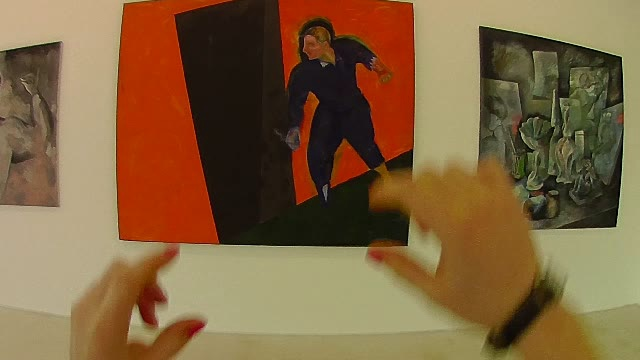
\includegraphics[width=0.2\linewidth]{Figures/take_a_picture_23956_24002_all43.jpg}
}
\caption{Sample gestures from the \datasetunimore{} dataset and the Maramotti dataset.}
\label{example-unimore}
\end{figure}

We then propose the \datasetunimore{} dataset, a gesture recognition dataset taken from the ego-centric perspective in a virtual museum environment. It consists of 700 video sequences, all shot with a wearable camera, in an interactive exhibition room, in which paintings and artworks are projected over a wall, in a virtual museum fashion (see figure \ref{example-unimore}). The camera is placed on the user's head and captures a 800 $\times$ 450, 25 frames per second 24-bit RGB image sequence. In this setting, five different users perform seven hand gestures: \textit{like}, \textit{dislike}, \textit{point}, \textit{ok}, \textit{slide left to right}, \textit{slide right to left} and \textit{take a picture}. Some of them (like the \textit{point}, \textit{ok}, \textit{like} and \textit{dislike} gestures) are statical, others (like the two \textit{slide} gestures) are dynamical. 
This dataset is very challenging since there is fast camera motion and users have not been trained before recording their gestures, so that each user performs the gestures in a slightly different way, as would happen in a realistic context. We have publicly released our dataset\footnote{\url{http://imagelab.ing.unimore.it/files/ego_virtualmuseum.zip}}.

%In the demo room setting, users perform gestures in front of a wall over which the works of art are projected. This setting is quite controlled: the illumination is constant, the art works are in low light, while hands are well illuminated. In the same way, in the \textit{museum} setting, users perform gestures in front of real artworks inside a museum. This is a realistic and very challenging environment: the illumination changes, other visitors are present and sometimes walk in. 
Since Ego Vision applications are highly interactive, their setup step must be fast (i.e. few positive examples can be acquired). Therefore, to evaluate the proposed gesture recognition approach, we train a 1-vs-1 linear classifier for each user using only two randomly chosen gestures per class as training set. The reported results are the average over 100 independent runs.

In Table \ref{gesture_comparison} we show the gesture recognition accuracy for each of the five subjects, and we also compare with the ones obtained without the use of the hand segmentation mask for camera motion removal and trajectories pruning.  Results show that our approach is well suited to recognize hand gestures in the ego-centric domain, even using only two positive samples per gesture, and that the use of the segmentation mask can improve recognition accuracy.


\begin{table}
\begin{center}
\renewcommand{\arraystretch}{1.3}
\centering
\begin{tabular}{|l|c|c|}
\hline
\textbf{User}							& \textbf{No segmentation} & \textbf{With segmentation}  \\
\hline
\hline
Subject 1				 			& 0.91 		& \textbf{0.95} \\
\hline
Subject 2			 				& 0.87 		& \textbf{0.87} \\
\hline
Subject 3					 		& 0.92		& \textbf{0.95}\\
\hline
Subject 4							& \textbf{0.96}	& 0.94 \\
\hline
Subject 5							& 0.91		& \textbf{0.96} \\
\hline
Average						&  0.91	& \textbf{0.93}  \\
\hline
\end{tabular}
\end{center}
\caption{Gesture recognition accuracy on the \datasetunimore{} dataset with and without hand segmentation.}
\label{gesture_comparison}
\end{table}

On a different note, to test our approach in a real setting, we created a dataset with videos taken in the Maramotti modern art museum, in which paintings, sculptures and \textit{objets d'art} are exposed. As in the previous dataset, the camera is placed on the user's head and captures a 800 $\times$ 450, 25 frames per second image sequence. The Maramotti dataset contains 700 video sequences, recorded by five different persons (some are the same of the Interactive Museum dataset), each performing the same gestures as before in front of different artworks. We have publicly released this dataset too\footnote{\url{ http://imagelab.ing.unimore.it/files/ego_maramotti.zip}}.
   
Figure \ref{example-unimore} show some examples of gestures performed in the two datasets. In the Interactive Museum dataset, users perform gestures in front of a wall over which the works of art are projected. This setting is quite controlled: the illumination is constant, the art works are in low light, while hands are well illuminated. On the other hand, in the Maramotti dataset, users perform gestures in front of real artworks inside a museum. This is a realistic and very challenging environment: the illumination changes, other visitors are present and sometimes walk in. In both cases there is significant camera motion, because the camera moves as the users move their heads or arms. It is also important to underline that users have not been trained before recording their gestures, so each user performs the gestures in a slightly different way, as would happen in a realistic context.  

In Table \ref{gesture_comparison_maramotti} we show the results of our gesture recognition approach on the Maramotti dataset. As can be seen, in this case the challenging and real environment causes a drop in accuracy. This is mainly due to the illumination changes, to the presence of other visitors, and to the fact that often the artworks are better illuminated than hands.
Since our wearable vision devices is fully connected to a central server, we show how the use of other visitors' gestures can improve the recognition accuracy.
In our scenario each visitor coming to the museum performs, in the initial setup phase, two training gestures for each class. These training gestures from past visitors, manually checked, are used to augment the training set, so no erroneous data is accumulated into the model. In particular, in our test ``Augmented'' (Table \ref{gesture_comparison_maramotti}) each ego-vision wearable device uses two randomly chosen gestures performed by its user as training, plus gestures performed by the remaining four users supplied by their devices to the central server. Results show that this distributed approach is effective and leads to a significant improvement in accuracy.


\begin{table}[tb]
\renewcommand{\arraystretch}{1.3}
\caption{Gesture recognition accuracy on the Maramotti dataset.}
\label{gesture_comparison_maramotti}
\centering
\begin{tabular}{|l|c|c|}
\hline
\textbf{User}					& \textbf{Single user's Gestures} 	& \textbf{Augmented}  \\
\hline
\hline
User A						& 0.54 			& \textbf{0.65} \\		% 4 Beppe
\hline
User B			 				& 0.52 			& \textbf{0.72} \\		% 2 Francesco
\hline
User C			 			& 0.68 			& \textbf{0.68} \\		% 1 Lorenzo
\hline
User F					 		& 0.56 			& \textbf{0.79} \\		% 3 Stefano
\hline
User G						& 0.53 			& \textbf{0.72} \\		% 5 Michela
\hline
\textbf{Average}					& 0.57	  		& \textbf{0.71} \\
\hline
\end{tabular}
\end{table}

We described a novel approach to cultural heritage fruition based on ego-centric vision devices. Our work is motivated by the increasing interest in ego-centric vision and by the growth of the cultural market, which encourages the development of new interfaces to interact with the cultural heritage. We presented a gesture and painting recognition model that can deal with static and dynamic gestures and can benefit from a distributed training. Our gesture recognition and hand segmentation results outperform the state-of-the-art approaches on Cambridge Hand Gesture and CMU EDSH datasets. Finally, we ran an extensive performance analysis of our system on a wearable board. 

In the next chapter, a real-time version of the described algorithm will be proposed, and we will describe the necessary optimizations steps to make such implementation real-time.

% Chapter 1

\chapter{A sequential implementation for the Odroid-XU developer board}

\lhead{Chapter 5. \emph{A sequential implementation}} % This is for the header on each page - perhaps a shortened title

%----------------------------------------------------------------------------------------
Finally, we turn our attention to define and implement a sequential version of our gesture recognition approach that can run in real-time on an embedded device and which could be suitable for real-world application. To this aim, we modify and improve the classification module of our gesture recognition algorithm, replacing the simple linear SVM classifier with a more complex Structural SVM implementation, designed to take into account time, and choose the Odroid-XU developer board as our target plaform. To make our implementation capable of running in real-time, we exploit several optimization techniques.

We evaluate the Structural SVM implementation by Altun \etal using feature vectors generated from our gesture recognition algorithm. We modify the source code provided by Joachims \cite{joachims} in order to include higher order label-label and label-features interactions, so that the generic 
$\Psi(\mathbf{x},\mathbf{y})$ takes the following form:

\begin{equation}
\Psi_{\epsilon,\tau}(\mathbf{x},\mathbf{y}) = \left( \begin{array}{cc} \sum_{t=1}^T \Phi(\mathbf{x}^t) \otimes  \Lambda^c(y^{t-\epsilon}) \otimes ... \otimes \Lambda^c(y^t) \\ \eta\sum_{t=1}^{T}  \Lambda^c(y^{t-\tau}) \otimes ... \otimes \Lambda^c(y^t) \end{array} \right)
\end{equation}

where $\epsilon$ is the order of label-label dependencies, and $\tau$ is the order of label-features dependencies.

Furthermore, we investigate the use of different loss functions and their impact on recognition rates and confusion matrices. We define a generic loss function that exploits a per-token loss function $\delta(y^t,y'^t)$: $\Delta(\mathbf{y},\mathbf{y'}) = \sum_{t=1}^T \delta(y^t,y'^t)$, and propose two different per-token loss functions:

\begin{equation}
\delta_0(y,y') = \begin{cases} 0 \quad \text{if } y= y'  \\ 
1 \quad \text{otherwise}\end{cases}
\end{equation}

\begin{equation}
\delta_1(y,y') = \begin{cases} 0 \quad \text{if } y= y'  \\ 
3 \quad \text{if } y=8, y' \neq 8 \lor y\neq8, y'=8  \\
1 \quad \text{otherwise}\end{cases}
\end{equation}

\section{The Odroid-XU board}
Our cultural heritage system consists of a collection of wearable ego-vision devices, that embed a glass-mounted camera and an Odroid-XU developer board, serving as video-processing and network communication unit.
There are several benefits in using such a portable device: the commercial availability and low costs for prototypes evaluation, the computational power and energy efficiency of the Big-Little architecture. Furthermore it has the possibility  of peripheral addition to extend connections and input devices. 

\begin{figure}[t!]
\centering
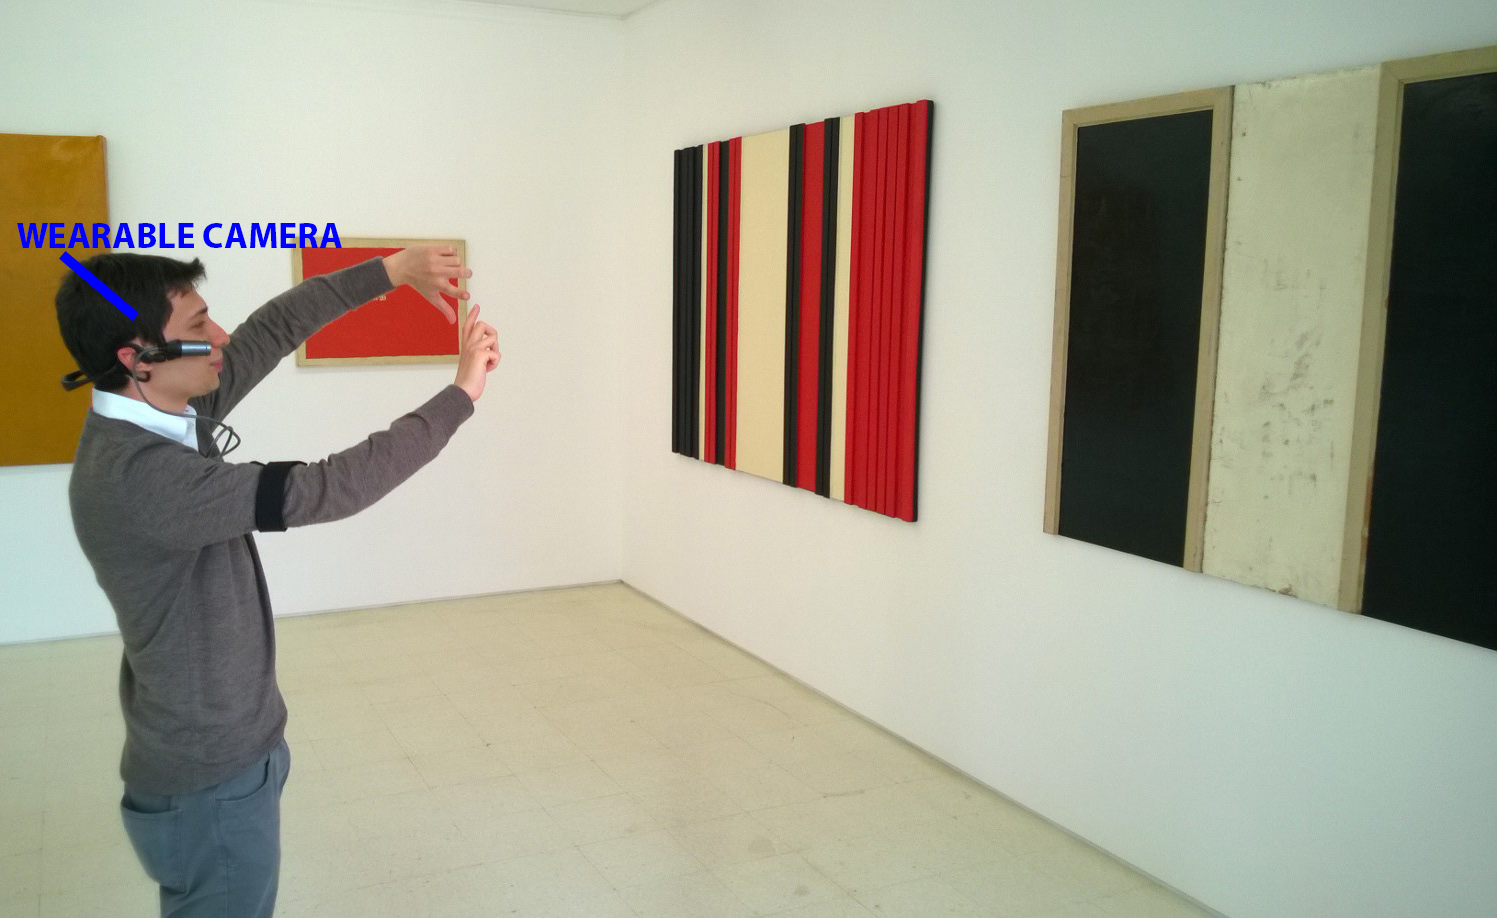
\includegraphics[width=0.5\linewidth]{Figures/lore_maramotti.jpg}
\caption{User interacting with wearable camera.}
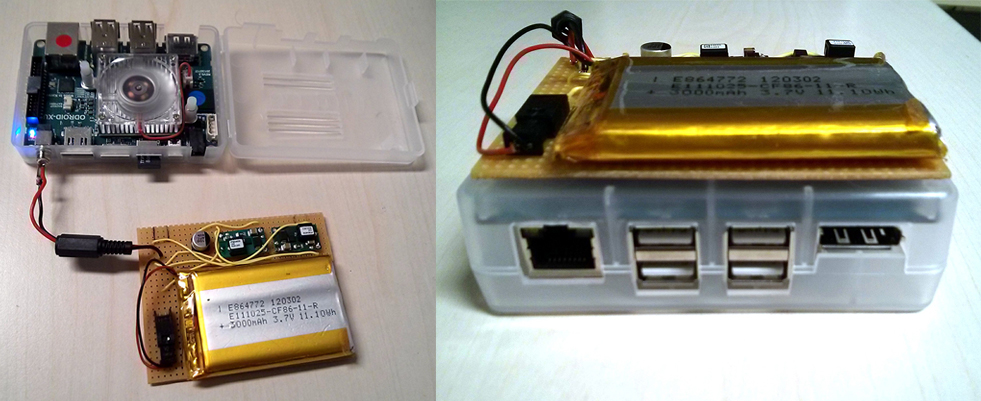
\includegraphics[width=0.5\linewidth]{Figures/board.jpg}

\caption{The Odroid-XU board with battery pack.}
\label{board}
\end{figure}

Hardkernel have made a name for themselves within the open-source community by delivering high performance development boards at affordable prices. The Odroid-XU platform boasts an Exynos 5 Octa processor – the same SoC found inside the Samsung Galaxy S4, which includes a PowerVR SGX544MP3 GPU clocked at around 600 MHz (see figure \ref{odroid-xu}).

The key features and specifications of the ODROID-XU development board include:
\begin{itemize}
\item big.LITTLE processing based on the Cortex™-A15 and Cortex™-A7 quad core CPUs
\item PowerVR SGX544MP3 GPU (OpenGL ES 2.0, OpenGL ES 1.1, OpenCL 1.1 EP, Renderscript/Filterscript)
\item 2Gbyte LPDDR3 PoP (1600Mbps/pin, 2 x 32bit Bus)
\item USB 3.0 Host x 1, OTG x 1, USB 2.0 Host x 4
\item HDMI 1.4a output Type-D connector (Micro-HDMI)
\item eMMC 4.5 Flash Storage
\item Micro-SD socket
\item MIPI DSI for LCD display output
\item On-board Audio Codec
\item Fast 10/100 Ethernet LAN
\item WiFi
\item 5V/4A power supply
\end{itemize}

Big.LITTLE is a heterogeneous computing architecture developed by ARM that couples slower, low-power processor cores with more powerful and power-hungry ones. The intention being to create a multi-core processor that can adjust better to dynamic computing needs and use less power than clock scaling alone. In this case we have the Cortex-A7 coupled with the Cortex-A15, which have been designed to be architecturally compatible.

In the Samsung Exynos 5 there is only one way for the different processor cores to be arranged in a big.LITTLE design: the \textit{clustered model} approach. With this approach the operating system scheduler can only see one of the two processor clusters, when the load on one cluster hits a certain point, the system transitions to the other cluster. All relevant data is passed through the common L2 cache, the first core cluster is powered off and the other one is activated. A Cache Coherent Interconnect (CCI) is used.




\begin{figure}[t!]
\centering
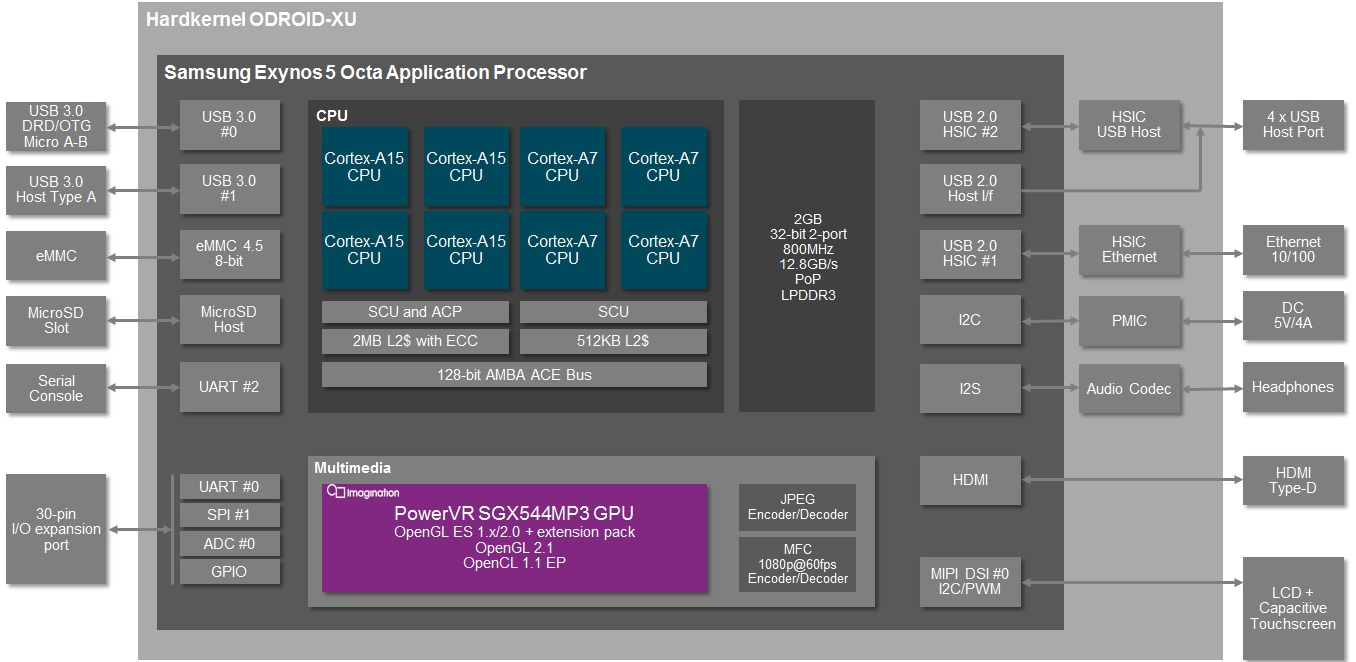
\includegraphics[width=0.9\linewidth]{Figures/Hardkernel-ODROID-XU-block_diagram.jpg}
\caption{Hardkernel Odroid-XU block diagram}
\label{odroid-xu}
\end{figure}

\section{Implementation}
\lstset{language=C++}

As stated before, on the Odroid-XU board only one of the two clusters can run at the same time. Since our application is heavy, we choose the A15 cluster, which includes four cores and is the most performant cluster. This is done trough the following command:
\begin{lstlisting}[frame=single]  % Start your code-block

echo performance > /sys/devices/system/cpu/cpu0/cpufreq/scaling_governor
\end{lstlisting}
which basically activates the \verb+performance+ governor as the controller for the big.LITTLE switching mechanism.
Then, having written a sequential implementation of our algorithm using the OpenCV library\footnote{This is joint work with Francesco Paci.}, we compile it using \verb+gcc+ with the following options:
\begin{lstlisting}[frame=single]  % Start your code-block

-g -mfpu=neon-vfpv4 -ftree-vectorize -mfloat-abi=hard -mtune=cortex-a15 -marm
\end{lstlisting}

The \verb+-g+ flag tells the compiler to produce debugging information in the operating system's native format, \verb+-mfpu=neon+  specifies what floating-point hardware (or hardware emulation) is available on the target, \verb+-ftree-vectorize+ enables the auto-vectorizer (which will try to use SIMD instructions, when possible), \verb+-mfloat-abi=hard+ allows generation of floating-point instructions and uses FPU-specific calling conventions, and \verb+-mtune=cortex-a15+ tunes the performance of the compiler for the A15 target.

\subsection{OpenMP and Neon Intrisics}
This first sequential version runs at 4.3 frames/s on $160\times 120$ frames, and needs 234 ms to elaborate each frame. The main bottleneck of this implementation is the multi-scale Farneback's optical flow, which requires 141 ms for each frame to run. Farneback's algorithm is executed two times for each frame, since the optical flow is calculated both on the original frame on the warped one, so we use OpenMP to run these two executions simultaneously on two different threads. Then, we use Neon intrinsics in order to exploit the SIMD capabilities of our CPU and thus gain a better performance on each thread.

A complete explanation of the optimizations made is beyond the purpose of this chapter, but, as an example, let's consider this for loop, which is responsible of 51 of the 234 ms:
\begin{lstlisting}[frame=single]  % Start your code-block

for( ; x < width*5; x++ ) {
	float s0 = srow[m][x]*kernel[0];
	for( i = 1; i <= m; i++ )
		s0 += (srow[m+i][x] + srow[m-i][x])*kernel[i];
	vsum[x] = s0;
}
\end{lstlisting}

Once optimized with Neon SIMD, the previous code becomes:
\begin{lstlisting}[frame=single]  % Start your code-block

int xstart = x;
float kernelext0[4];
fill_n(kernelext0,4,kernel[0]);
for( ; x < width*5-4; x+=4 ) {
           vst1q_f32(vsum+x, vmulq_f32(vld1q_f32(srow[m]+x),
		vld1q_f32(kernelext0)));
}
float a[width*5];
float kernelext[4];
for( i = 1; i <= m; i++ ) {
	fill_n(kernelext, 4, kernel[i]);
           for (x=xstart; x<width*5-4; x+=4) {
                        vst1q_f32(a+x, vaddq_f32(vld1q_f32(srow[m+i]+x), 
			vld1q_f32(srow[m-i]+x)));
                        vst1q_f32(vsum+x, vmlaq_f32(vld1q_f32(vsum+x), 
			vld1q_f32(a+x), vld1q_f32(kernelext)));
           }
}
\end{lstlisting}
As can be seen, the two for loops have been inverted and four floats are processed at each iteration. The new code block takes only 20 ms to run. 

\subsection{Further optimizations}
Having included several OpenMP/SIMD optimizations, our code runs at 7.1 frames/s on the A15 cluster, still not enough for real-time. Moreover, our algorithm needs an high frame rate in order to compute significant trajectories. Being the Farneback's algorithm our main bottleneck, we could turn our attention to the PowerVR GPU embedded into the Odroid board. Unfortunately, Hardkernel has not yet released an Ubuntu kernel that supports the PowerVR GPU\footnote{see: \url{http://forum.odroid.com/viewtopic.php?f=61&t=2236}.}, so the only way we have to increase speed is to further reduce the frame size and keep only one level of the spatial pyramid. Having reduce the frame size to $113\times 85$


... the Farneback's optical flow\footnote{\url{https://github.com/Itseez/opencv/blob/9aa4410509fcc60dfabb78c14a96ed5153ee117e/modules/ocl/src/opencl/optical_flow_farneback.cl}} is included in the C++ code.


\section{Some applications}
\subsection{Ego-Vision Jacket}
\subsection{...}


\chapter{Conclusion}

%----------------------------------------------------------------------------------------
%	THESIS CONTENT - APPENDICES
%----------------------------------------------------------------------------------------

\addtocontents{toc}{\vspace{2em}} % Add a gap in the Contents, for aesthetics

\appendix % Cue to tell LaTeX that the following 'chapters' are Appendices

% Include the appendices of the thesis as separate files from the Appendices folder
% Uncomment the lines as you write the Appendices

% Appendix A

\chapter{Publications} % Main appendix title

\label{AppendixA} % For referencing this appendix elsewhere, use \ref{AppendixA}

\lhead{Appendix A. \emph{Publications}} % This is for the header on each page - perhaps a shortened title

The research activity conducted in the context of this thesis has led to some publications in international journals
and workshops. These are summarized below.

\begin{enumerate}
\item \textbf{L. Baraldi}, S. Alletto, G. Serra, R. Cucchiara. ``Interacting with Art: Ego-vision for Enriched Cultural Experience'', \textit{Machine Vision and Applications}. (Submitted)
\item \textbf{L. Baraldi}, F. Paci, G. Serra, L. Benini, R. Cucchiara. ``Gesture Recognition using Wearable Vision Sensors to Enhance Visitors’ Museum Experiences'', \textit{IEEE Sensors Journal}. (Submitted after minor revision)
\item \textbf{L. Baraldi}, F. Paci, G. Serra, L. Benini, R. Cucchiara. ``Gesture Recognition in Ego-Centric Videos using Dense Trajectories and Hand Segmentation'', in \textit{IEEE Computer Vision and Pattern Recognition (CVPR) Embedded Vision Workshop (EVW)}, 2014.
\item G. Serra, M. Camurri, \textbf{L. Baraldi}, M. Benedetti, R. Cucchiara. ``Hand Segmentation and Gesture Recognition in EGO-Vision'', in \textit{Proc. of ACM Multimedia International Workshop on Interactive Multimedia on Mobile and Portable Devices (IMMPD)}, 2013.
\end{enumerate}
%\input{Appendices/AppendixB}
%\input{Appendices/AppendixC}

\addtocontents{toc}{\vspace{2em}} % Add a gap in the Contents, for aesthetics

\backmatter

%----------------------------------------------------------------------------------------
%	BIBLIOGRAPHY
%----------------------------------------------------------------------------------------

\label{Bibliography}

\lhead{\emph{Bibliography}} % Change the page header to say "Bibliography"

\bibliographystyle{unsrtnat} % Use the "unsrtnat" BibTeX style for formatting the Bibliography

\bibliography{Bibliography} % The references (bibliography) information are stored in the file named "Bibliography.bib"


\end{document}  

